\PassOptionsToPackage{usenames,dvipsnames,table,x11names}{xcolor}
\documentclass[8pt]{beamer}

% SETTING THEMES ----------------------------------------
%\usetheme{Warsaw}
\usetheme{Luebeck}
%\usetheme{Boadilla}

% COLORS IN PRESENTATION --------------------------------
\setbeamercolor*{palette primary}{bg = Firebrick1, fg = white}
%\usepackage{color}


%https://www.tug.org/pracjourn/2007-4/walden/color.pdf
%https://tex.stackexchange.com/questions/368784/change-color-in-beamer-theme

% FONT --------------------------------------------------
%\usefonttheme{professionalfonts} %doesn't do anything?
\usefonttheme{serif}

% CHANGING ITEMIZE ITEMS --------------------------------
\setbeamertemplate{itemize item}{\color{black} $\vcenter{\hbox{\tiny$\bullet$}}$} %style of item
\setbeamertemplate{itemize subitem}{\tiny \color{white}$\blacktriangleright$} %style for sub item
\setbeamercolor{itemize item}{fg=black} %changes color of all items

\setbeamertemplate{enumerate items}[default] %default number style
\setbeamercolor{enumerate item}{fg=black}

%\setbeamerfont{frametitle}{size=\Large}

%https://tex.stackexchange.com/questions/59742/progress-bar-for-latex-beamer

%\insertframenumber/\inserttotalframenumber

%getting rid of stuff on bottom
\setbeamertemplate{footline}[frame number]{}
\setbeamertemplate{navigation symbols}{}
%\setbeamertemplate{footline}{%
%    \raisebox{5pt}{\makebox[\paperwidth]{\hfill\makebox[20pt]{\color{gray}
%          \scriptsize\insertframenumber/\inserttotalframenumber}}}\hspace*{5pt}}

%\usepackage{natbib}
%\renewcommand\bibfont{\scriptsize}
\setbeamercolor*{bibliography entry title}{fg=black}
\setbeamercolor*{bibliography entry author}{fg=black}
\setbeamercolor*{bibliography entry location}{fg=black}

%\newcommand*{\myfont}{\fontfamily{phv}\selectfont} %helvecta
%\newcommand*{\myfont}{\fontfamily{crm}\selectfont} %cm wont change
%https://tex.stackexchange.com/questions/25249/how-do-i-use-a-particular-font-for-a-small-section-of-text-in-my-document

%%%%%%%%%%%%%%%%%%%%%%%%%%%%%%%%%%%%%%%%%%%%%%%%%%%%%%%%%%
%%%%%%%%%%%%%%%%%%%%%%%%%%%%%%%%%%%%%%%%%%%%%%%%%%%%%%%%%%
%%%%%%%%%%%%%%%%%%%%%%%%%%%%%%%%%%%%%%%%%%%%%%%%%%%%%%%%%%

%------------------------------------------------------
%                Math Packages
%------------------------------------------------------

%\usepackage[intlimits]{amsmath}
\usepackage{amsmath}
\usepackage{amssymb}
\usepackage{amsthm}
%\everymath{\displaystyle}
\usepackage{siunitx} % for SI units (e.g. C, degree)
\usepackage{bm} % bold for some math symbols
\usepackage{nicefrac} % for nicer fractions sometimes
\usepackage[thinc]{esdiff} % for derivatives

%------------------------------------------------------
%                Tikz and Pgfplots
%------------------------------------------------------

\usepackage{pgfplots}
\usepackage{tkz-euclide}
\pgfplotsset{compat=1.15}
\usetikzlibrary{arrows,shadows,positioning, calc, decorations.markings, hobby, quotes,angles,decorations.pathreplacing,intersections, matrix,backgrounds}
\usepgfplotslibrary{polar,colormaps,fillbetween}
\usepgflibrary{shapes.geometric}
%\usetkzobj{all}

%------------------------------------------------------
%                Formatting
%------------------------------------------------------

% COLORS ----------------------------------------------
%\usepackage[dvipsnames, table]{xcolor}
\usepackage{xcolor}

% FIGURES ---------------------------------------------
\usepackage{graphicx} % for importing images
\usepackage{subcaption} % for making subfigures
\usepackage[labelfont=bf]{caption} % changing style of figures
% use font=it for italic font

% PAGE LAYOUT -----------------------------------------
%\linespread{1.3} % changes line spacing
\setlength{\parskip}{0.25em}
\setlength{\itemsep}{0.25em}

%\usepackage{indentfirst}
%\usepackage{parskip} % for not indenting paragraphs first
\usepackage{multirow} % having multiple rows
\usepackage{multicol} % having multiple columns
\usepackage[T1]{fontenc} % can combine \sc and \bf font

% LANGUAGES -------------------------------------------
\usepackage[english]{babel} % for correctly using english
\usepackage[utf8x]{inputenc} % compiling correctly
\usepackage{CJK} % using Chinese, Japanese, and Korean

% MISC ------------------------------------------------
\usepackage[normalem]{ulem} % for \sout
\usepackage{tikzsymbols} % for emojis
\usepackage{booktabs,eqparbox} % for tables
\usepackage{verbatim} % for verbatim environment
%\usepackage{xmpmulti} % for animations
\usepackage{media9} % for animations
\usepackage{animate} % for animations

% CITING ----------------------------------------------
\usepackage{apacite}
%\newcommand{\citeay}[1]{\citeauthor{#1} \citeyear{#1}}

%------------------------------------------------------
%                Custom Commands
%------------------------------------------------------

\newcommand{\done}{\hfill $\square$ \vspace{1cm}}
\newcommand{\csch}{\mathrm{csch}}
\newcommand{\sech}{\mathrm{sech}}

%\newcommand{\dd}{\mathop{}\,\mathrm{d}}
\newcommand{\dd}{\;\mathrm{d}}

% COLOR CODING -----------------------------------------------
\newcommand{\code}[1]{\textcolor{Bittersweet}{\texttt{#1}}} % using for emphasizing variables, code, etc.
\newcommand{\mydef}[1]{\textcolor{SteelBlue3}{\textit{#1}}} % defining something

% VENN DIAGRAMS ----------------------------------------------
\def\firstcircle{(90:1.75cm) circle (2.5cm)}
\def\secondcircle{(210:1.75cm) circle (2.5cm)}
\def\thirdcircle{(330:1.75cm) circle (2.5cm)}
\def\sampspace{(-6,-4.25) rectangle (6,5)}  %Cartesian
%\def\sampspace{(225:7cm) rectangle (45:7cm)} %polar

% TO DO LIST -------------------------------------------------
%\usepackage{enumitem}

%\newlist{todolist}{itemize}{2}
%\setlist[todolist]{label=$\square$}

%\usepackage{pifont}
%\newcommand{\cmark}{\ding{51}}%
%\newcommand{\xmark}{\ding{55}}%
%\newcommand{\fin}{\rlap{$\square$}{\raisebox{2pt}{\color{Green}{\large\hspace{1pt}\cmark}}}%
%\hspace{-2.5pt}}
%\newcommand{\wontfix}{\rlap{$\square$}{\color{red}{\large\hspace{1pt}\xmark}}}

%------------------------------------------------------
%                Custom Environments
%------------------------------------------------------

\usepackage{mdframed}

% EXERCISE -------------------------------------------------
\mdfdefinestyle{exercise}{
	backgroundcolor=black!10,roundcorner=8pt,hidealllines=true,nobreak
}

%\begin{mdframed}[style=exercise]
%\end{mdframed}

% MATHEMATICA ------------------------------------------------
\mdfdefinestyle{mathematica}{
	backgroundcolor=Tan!15,roundcorner=8pt,hidealllines=true,nobreak,fontcolor=Bittersweet
}

% R ---------------------------------------------------------
\mdfdefinestyle{R}{
	backgroundcolor=SteelBlue3!15, roundcorner=8pt, hidealllines=true, nobreak, fontcolor=SteelBlue3
}

% R ---------------------------------------------------------
\mdfdefinestyle{python}{
	backgroundcolor=Green!15, roundcorner=8pt, hidealllines=true, nobreak, fontcolor=Green
}

%\usepackage[style=authoryear]{biblatex}

%%%%%%%%%%%%%%%%%%%%%%%%%%%%%%%%%%%%%%%%%%%%%%%%%%%%%%%%%%
%%%%%%%%%%%%%%%%%%%%%%%%%%%%%%%%%%%%%%%%%%%%%%%%%%%%%%%%%%
%%%%%%%%%%%%%%%%%%%%%%%%%%%%%%%%%%%%%%%%%%%%%%%%%%%%%%%%%%

% change this to add pauses in the presentation

\newcommand{\mys}{\vspace{0.5cm} %\pause
}
\newcommand{\mysa}{\vspace{0.2cm} %\pause
}

\title{Sparse Regression with Clustered Predictors}
\author{Aiden Kenny and Danielle Solomon}
\institute{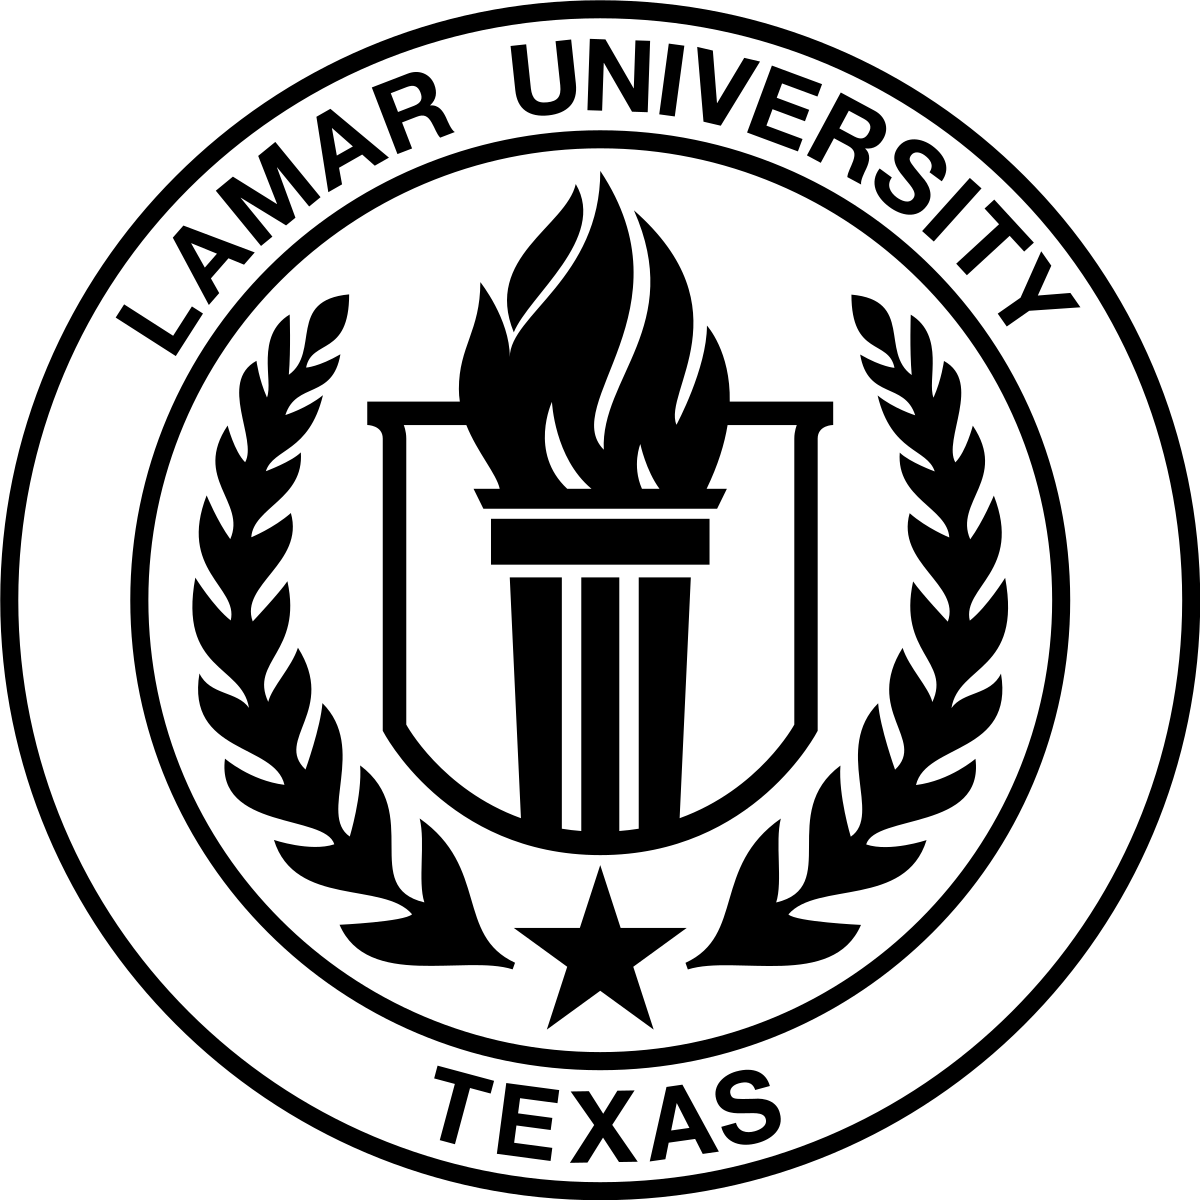
\includegraphics[width = 0.25\textwidth]{lamar_seal.png}}
\date{Research Experience for Undergraduates\\[0.5pt]
Mentor: Dr. Kumer Das\\[0.5pt]
Lamar University\\[0.5pt]
August 9, 2019}
    
\begin{document}

%%%%%%%%%%%%%%%%%%%%%%%%%%%%%%%%%%%%%%%%%%%%%%%%%%%%%%%%%%
%%%%%%%%%%% TITLE FRAME %%%%%%%%%%%
%%%%%%%%%%%%%%%%%%%%%%%%%%%%%%%%%%%%%%%%%%%%%%%%%%%%%%%%%%

\begin{frame}

\maketitle

\end{frame}

\begin{frame}{Introduction}

\textit{Statistical learning} involves using collected data to build a statistical model that can predict a \textit{response} given a set of \textit{predictors}.
\begin{itemize} 
    \item e.g. Given the gene expression for $2000$ genes, we want to predict if a person has cancer or not.
    \item The applications are endless!
\end{itemize} \mys 

When building statistical models, people look for two things:
\begin{enumerate}
    \item \textit{Model accuracy}: given an input, we want to correctly predict the outcome.
    \item \textit{Model interpretability}: of all of the predictors we have, which ones are the most important?
\end{enumerate} \mys

Many data sets are \textit{high-dimensional}, meaning the number of predictors is much larger than the number of observations.
\begin{itemize}
    \item e.g. You only observe $62$ patients, but have $2000$ genes for each one.
    \item In this setting, traditional statistical models no longer suffice.
\end{itemize} 

\end{frame}

\begin{frame}{\color{white}$\ldots$}

\textit{Regularization} is used to improve upon traditional statistical models.
\begin{itemize}
    \item Prediction accuracy is improved.
    \item \textit{Sparse models} are models where many of the predictors are not significant to the response.
    \item Because regularization (sometimes) induces sparsity, the models are very interpretable.
    \item In the high-dimensional setting, simple models that are heavily regularized are favorable.
\end{itemize} \mys

There are many times where the predictors have a \textit{group} structure. 
\begin{itemize}
    \item e.g. The genes used to predict cancer belong to gene pathways.
    \item Basic regularization may perform poorly in this setting, both in terms of prediction accuracy and interpretability.
    \item Using this grouping information, we can improve both prediction accuracy and interpretability.
\end{itemize} %\mys

%Using this grouping information, we can improve both prediction accuracy and interpretability.
%\begin{itemize}
%    \item The response can be based off of the collective output of each group.
%    \item Now we can determine which \textit{groups} are important to the response, as opposed to which individual predictors.
%\end{itemize}
    
\end{frame}

\begin{frame}{$\ldots$}

However, a lot of times \textit{we do not know if there is a grouping structure beforehand}. 
\begin{itemize}
    \item This can be very bad if there truly is a grouping structure for the predictors.
\end{itemize} \mys

\textbf{Our objective}: to identify the grouping structure beforehand to improve our models. \mys

\textbf{How we do it}: we first use \textit{clustering} to define the predictor groups. Once these groups are defined, we fit a regularized model. \mys 

\textbf{Did it work?}: sometimes! It depends on how the groups are defined.
    
\end{frame}

\begin{frame}{\color{white} Notation}

The number of observations in a data set is denoted as $N$, and the number of predictors is denoted as $P$.
\begin{itemize}
    \item Let $\bm{x}_i \in \mathbb{R}^P$ denote the $i$th observation, for $i = 1, \ldots, N$.
    \item Let $\mathbf{x}_j \in \mathbb{R}^N$ denote the $j$th predictor, for $j = 1, \ldots, P$.
\end{itemize} \mys

We store the items in the \textit{data matrix} $\mathbf{X} \in \mathbb{R}^{N \times P}$.
\begin{itemize}
    \item The observations $\bm{x}_i$ are the \textit{rows} of $\mathbf{X}$, i.e. $\bm{x}_i = (x_{i, 1}, \ldots, x_{i, P})$
    \item The predictors $\mathbf{x}_j$ are the \textit{columns} of $\mathbf{X}$, i.e. $\mathbf{x}_j = (x_{1,j}, \ldots, x_{N,j})$.
\end{itemize} \mys

Let $x_{i,j}$ denote the value of the $j$th predictor for the $i$th observation.
\begin{itemize}
    \item Then we can write $\mathbf{X}$ as 
    \begin{align*}
        \mathbf{X} = \begin{pmatrix}
        x_{1,1} & \cdots & x_{1,P} \\
        \vdots & \ddots & \vdots \\
        x_{N,1} & \cdots & x_{N,P}
        \end{pmatrix}.
    \end{align*}
\end{itemize} \mys

Let $\mathbf{y} = (y_1, \ldots, y_n) \in \mathbb{R}^N$ be the response for each observation.
    
\end{frame}

\begin{frame}{Types of Statistical Learning}

In statistical learning, the response can either be \textit{continuous} or \textit{categorical}.
\begin{itemize}
    \item Predicting continuous responses is known as \textit{regression}, while predicting categorical responses is known as \textit{classification}.
    \item Continuous response takes on numerical values, while categorical responses take on class values.
    \item e.g. Given the sea level height every day for the past 20 years, we want to predict the sea level height in 2050. (continuous)
    \item e.g. Given the expression of 2000 genes, we want to predict if a person has cancer or not. (categorical)
\end{itemize} \mys

Throughout this presentation, we will use the colon data set as a motivating example.
\begin{itemize}
    \item This was one of the two real-world data sets used in our report.
    \item The expression of 2000 genes ($P=2000$) is measured for 62 different tissue samples ($N = 62$).
    \item The response is either a tissue sample has no cancer (occurred 22 times) or has cancer (occurred 40 times).
\end{itemize}
    
\end{frame}

\begin{frame}{\color{white} The Binary Setting}

For many classification problems, there are only two classes that the response can chose from.
\begin{itemize}
    \item We code the response as $y_i \in \{ 0,1 \}$.
    \item e.g. A tissue sample either does not have cancer ($y_i = 0$) or does have cancer ($y_i = 1$).
    \item This setting was the main focus of our research. 
\end{itemize} \mys 

Here (and for classification in general), we want to predict the \textit{probability} that an observation falls into either class.
\begin{itemize}
    \item Let $p(\bm{x}_i) = \mathbb{P}(Y = 1 \mid X = \bm{x}_i)$ be the probability that the $i$th observation belongs to class 1.
    \item Then we model the response as 
    \begin{align*}
        \hat{y}_i = \begin{cases}
        1, & \text{if } p(\bm{x}_i) \ge 0.5 \\
        0, & \text{if } p(\bm{x}_i) < 0.5
        \end{cases}.
    \end{align*}
\end{itemize}
    
\end{frame}

\begin{frame}{Logistic Regression}

\textit{Logistic regression} models $p(\bm{x}_i)$ using the \textit{log-odds}, given by
\begin{align}
    \label{logisticregression}
    \eta(\bm{x}_i) = \log \left( \frac{p(\bm{x}_i)}{1 - p(\bm{x}_i)} \right) = \beta_0 + \sum_{j=1}^P \beta_j x_{i, j}.
\end{align} \mysa

It assumes that the log-odds $\eta(\bm{x}_i)$ is a linear combination of the predictors.
\begin{itemize}
    \item The coefficients $\beta_1, \ldots, \beta_P$ determine the effect that each predictor has on $\eta(\bm{x}_i)$.
    \item If $\beta_j = 0$, then the $j$th predictor has no effect.
\end{itemize} \mys

Let $\bm{\beta} = (\beta_1, \ldots, \beta_P)$. Then we can re-write (\ref{logisticregression}) as $\eta(\bm{x}_i) = \beta_0 + \bm{x}_i^T \bm{\beta}$.

    
\end{frame}

\begin{frame}{\color{white} Fitting the model}

We are given a set of observations $(\bm{x}_i, y_i)$, for $i = 1, \ldots, N$, and from that we want to determine the coefficients $\beta_0$ and $\bm{\beta}$. \mys

We determine the coefficients by minimizing the \textit{negative log-likelihood}, given by 
\begin{align}
    \label{negloglike}
    L(\beta_0, \bm{\beta}) = \frac{1}{N} \sum_{i = 1}^N \Big[ \log \left(1 + e^{\eta(\bm{x}_i)}  \right)  - y_i \cdot \eta(\bm{x}_i) \Big].
\end{align}
\begin{itemize}
    \item $L(\beta_0, \bm{\beta})$ is a function of the coefficients. As we change $\beta_0$ and $\bm{\beta}$, we change the value of $L(\beta_0, \bm{\beta})$.
    \item We want to find the values of $\beta_0$ and $\bm{\beta}$ that give us the \textit{global (absolute) minimum} of $L(\beta_0, \bm{\beta})$.
    \item $L(\beta_0, \bm{\beta})$ is convex, which means that it has a global minimum that can be found efficiently!
\end{itemize}
    
\end{frame}

\begin{frame}{\color{white} $\ldots$}

\begin{columns}

\column{0.65\textwidth}
\begin{figure}
    \centering
    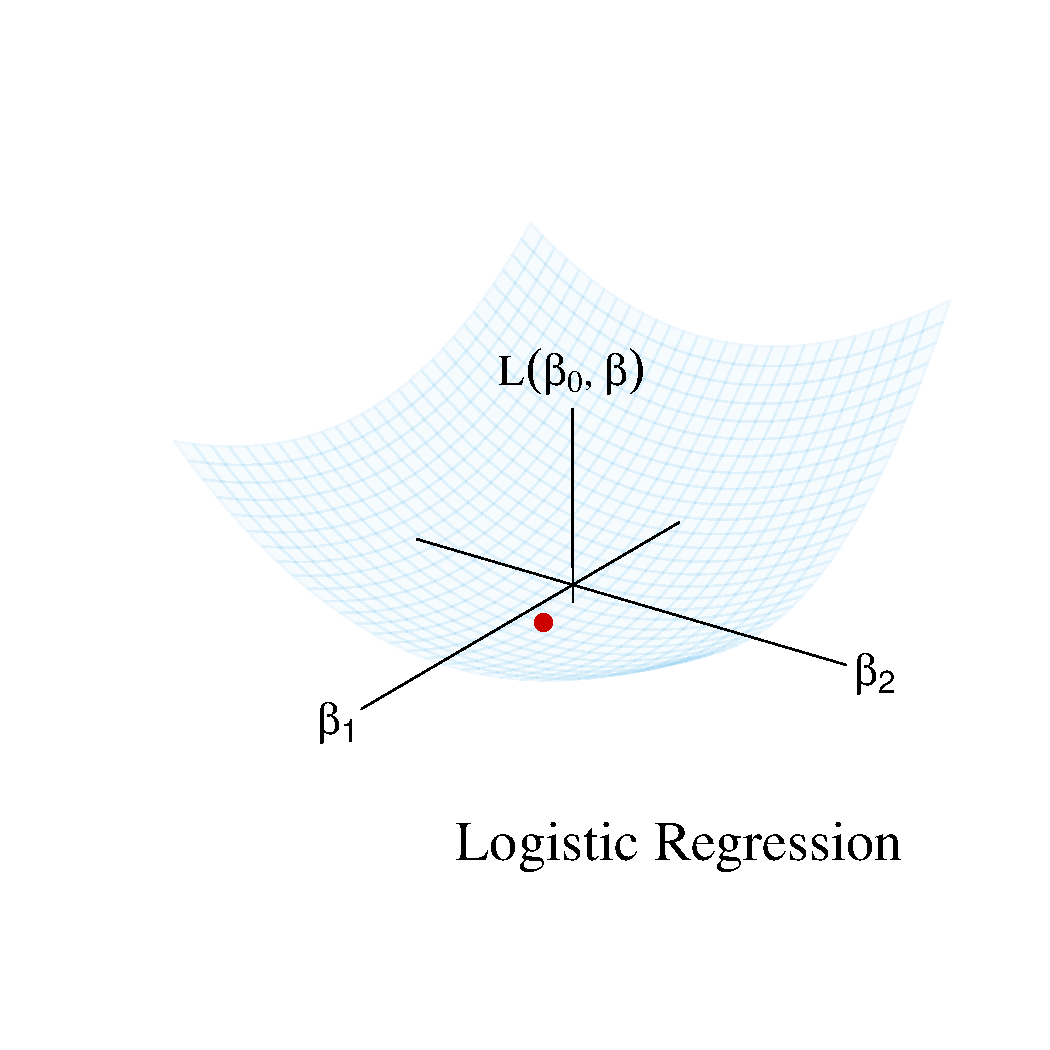
\includegraphics[trim = 0 0 0 0, clip, width = \textwidth]{min_nll.pdf}
\end{figure}

\column{0.35\textwidth}

In the special case of two predictors, we have $\bm{\beta} = (\beta_1, \beta_2)$. \mys

Here we plot $L(\beta_0, \bm{\beta})$ for a fixed value of $\beta_0$.
\begin{itemize}
    \item Assume that we have already found the optimal $\beta_0$.
    \item It will make sense why we are doing this shortly!
\end{itemize} \mys

The red dot indicates the value of $\bm{\beta}$ that minimizes $L(\beta_0, \bm{\beta})$!
    
\end{columns}
    
\end{frame}

\begin{frame}{Model Effectiveness}

For classification, we have two ways to measure how effective our model is:
\begin{enumerate}
    \item \textit{Deviance}, given by 
    \begin{align*}
        D(\beta_0, \bm{\beta}) = 2 \cdot L(\beta_0, \bm{\beta}).
    \end{align*}
    \item \textit{Error rate}, given by 
    \begin{align*}
        \mathrm{error} = \frac{1}{N} \| \hat{\mathbf{y}} - \mathbf{y}\|_1 = \frac{1}{N} \sum_{i=1}^N \mathbb{I}(\hat{y}_i \not = y_i).
    \end{align*}
\end{enumerate} \mys

Deviance is preferred since it is a more sensitive measurement.
\begin{itemize}
    \item e.g. For two models, suppose $p(\bm{x}_i) = 0.99$ and $p(\bm{x}_i) = 0.51$.
    \item We are much more confident in the first model, but for both models, the error rate will be the same.
\end{itemize} %\mys

%We fit a model with a training set and a test set.
%\begin{itemize}
%    \item The 
%\end{itemize}
    
\end{frame}

\begin{frame}{\color{white} The Bias-Variance Trade-Off}

There are two important properties about any statistical model:
\begin{enumerate}
    \item \textit{Bias}: the types of models we \textit{assume} can be fit.
    \item \textit{Variance}: how different the fitted model can be when we use different data.
    \item Too much bias $\to$ model under-fits.
    \item Too much variance $\to$ model over-fits.
\end{enumerate} \mys

We want to find a good balance between both. This is known as the \textit{bias-variance trade-off}:
\begin{align*}
    \mathbb{E}\Big(D(\beta_0, \bm{\beta} \mid \bm{x}_i, y_i)\Big) \propto \mathbb{B}\big(\eta(\bm{x}_i) \big)^2 + \mathbb{V}\big(\eta(\bm{x}_i) \big),
\end{align*}
where $\mathbb{E}(\cdot)$ is the expected value, $\mathbb{B}(\cdot)$ is the bias, and $\mathbb{V}(\cdot)$ is the variance. 
\begin{itemize}
    \item Put simply, the expected error depends on the bias and the variance. Too much of either is not good.
\end{itemize}\mys

In the high-dimensional setting, fitted logistic regression models will have very high variance! \Sadey[1.5][yellow]
    
\end{frame}

\begin{frame}{Regularization}

\textit{Regularization} involves minimizing a penalized version of $L(\beta_0, \bm{\beta})$, taking the general form 
\begin{align*}
    Q(\beta_0, \bm{\beta}) = L(\beta_0, \bm{\beta}) + \lambda P(\bm{\beta}).
\end{align*}
\begin{itemize}
    \item $P(\bm{\beta})$ is some type of \textit{penalty} that is imposed on $\bm{\beta}$.
    \item $\lambda$ is a tuning parameter that controls the severity of the penalty.
    \item As $\lambda \to \infty$, the penalty becomes more severe.
    \item Notice that we are not penalizing $\beta_0$.
\end{itemize} \mys 

This has the effect of limiting the size of the coefficients $\bm{\beta}$.
\begin{itemize}
    \item By doing so, we are adding more bias to the model.
    \item We hope that adding a \textit{small} amount of bias will result in a \textit{large} decrease in variance.
    \item This will improve prediction accuracy! 
\end{itemize}
    
\end{frame}

\begin{frame}{Model Flexibility}

\begin{figure}
    \centering
    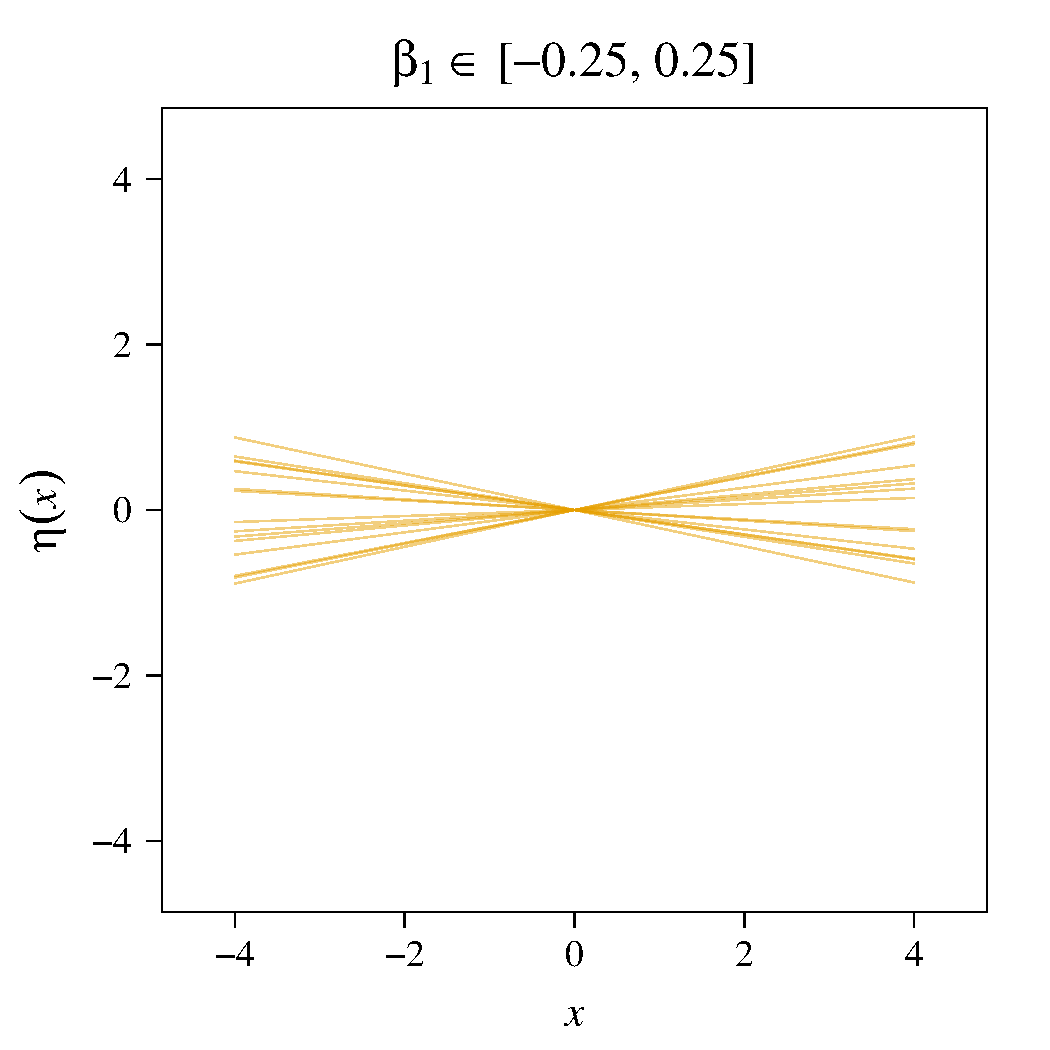
\includegraphics[width = 0.33\textwidth]{b1.pdf}
    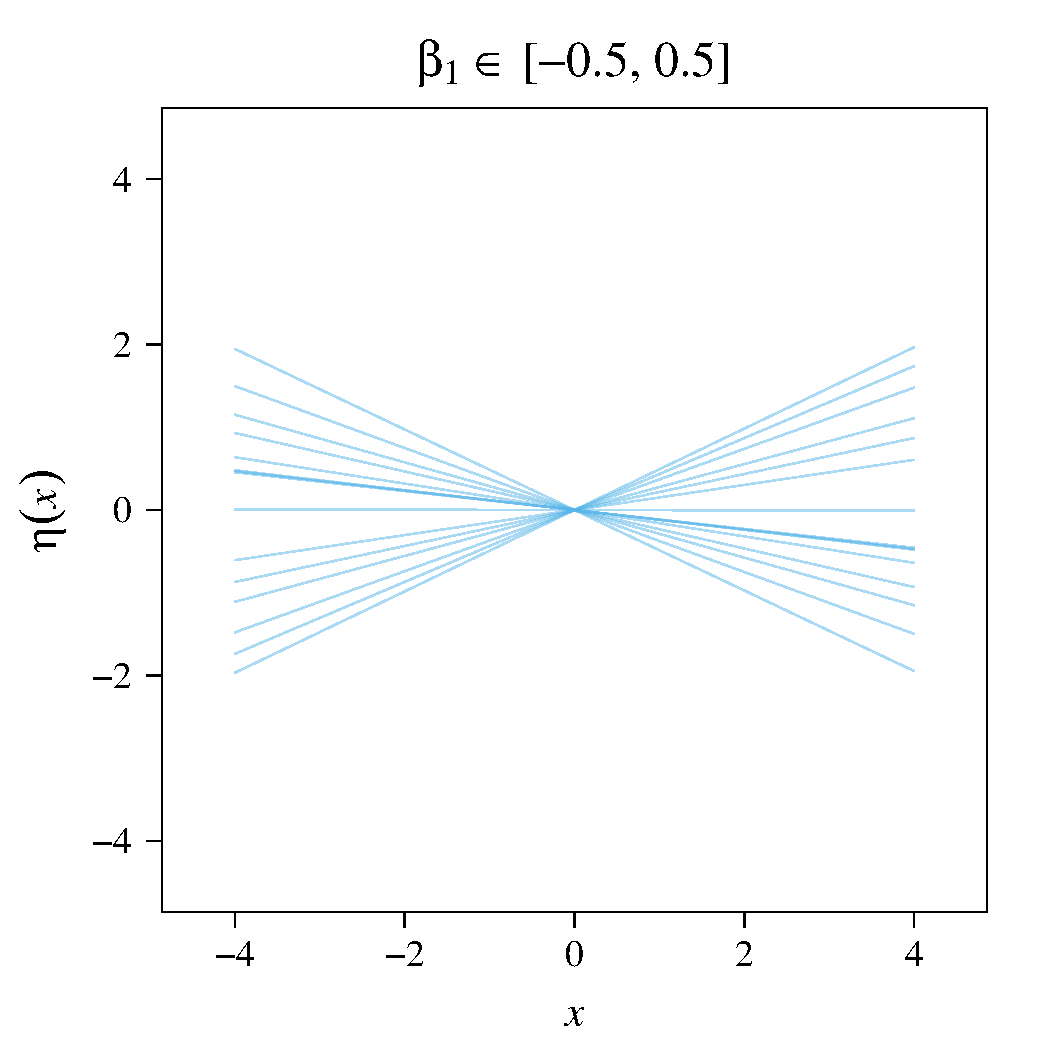
\includegraphics[width = 0.33\textwidth]{b2.pdf}
    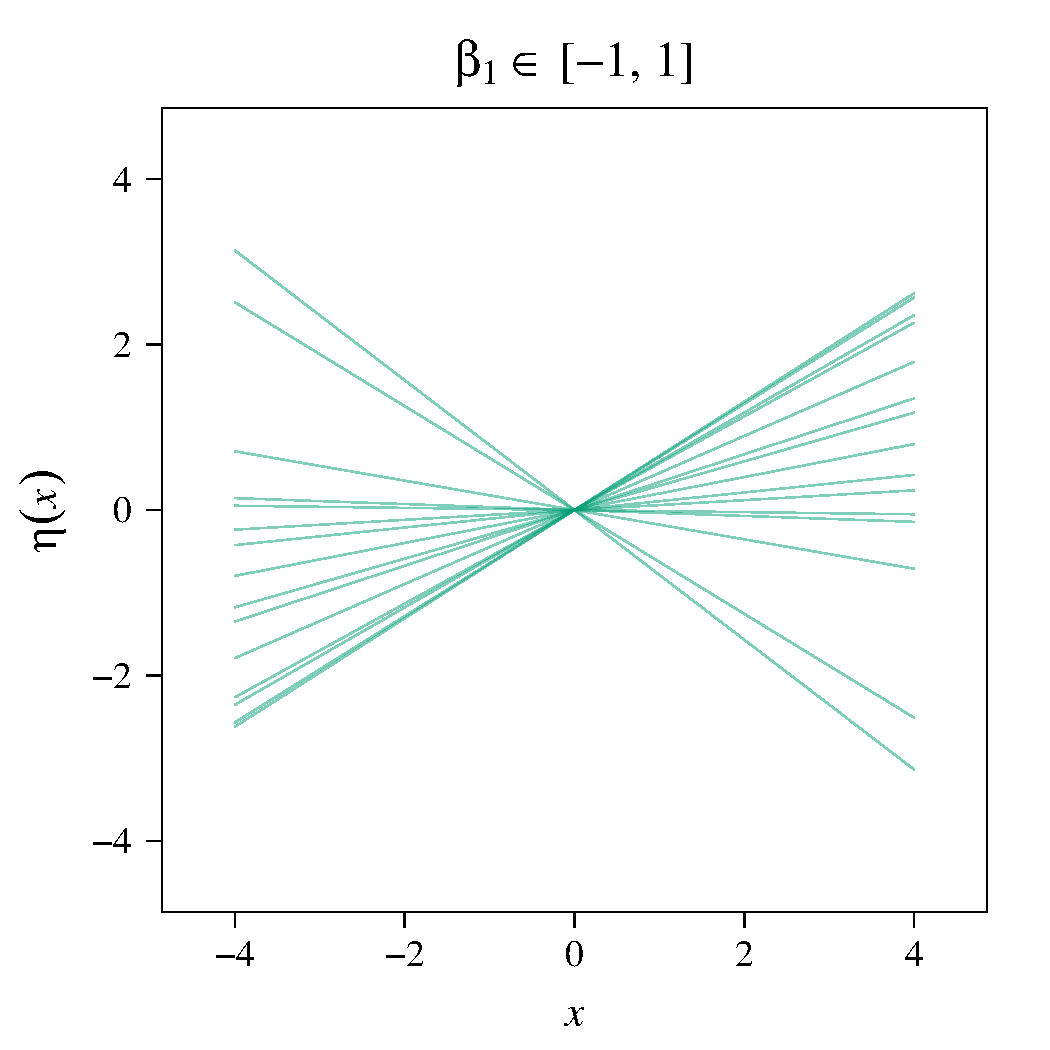
\includegraphics[width = 0.33\textwidth]{b3.pdf}
\end{figure}

Here is a simple example with \textit{one} predictor. So $\eta(x) = \beta_0 + \beta_1 x$.
\begin{itemize}
    \item For each picture, we are assuming that $\beta_1$ can take on an increasing range of values $\to$ we are assuming less about the model (bias decreasing).
    \item As this range increases, it is possible for the models to have steeper slopes $\to$ more types of models can be fit (variance increasing).
    \item Regularization shrinks this range of values, introducing bias and lowering variance.
\end{itemize}
    
\end{frame}

\begin{frame}{\color{white} Ridge Regression}

\textit{Ridge regression} minimizes 
\begin{align}
    \label{ridge regression}
    Q(\beta_0, \bm{\beta}) = L(\beta_0, \bm{\beta}) + \frac{\lambda}{2} \| \bm{\beta} \|_2^2.
\end{align} \mysa

The squared $\ell_2$ norm penalty $\| \cdot \|_2^2$ \textit{continuously} shrinks the coefficients.
\begin{itemize}
    \item The coefficients of highly-correlated predictors are shrunken together.
    \item This is what greatly reduces the variance.
\end{itemize} \mys

A major drawback to ridge regression is that \textit{none of the coefficients will equal 0}.
\begin{itemize}
    \item This is bad for model interpretability.
    \item e.g. The logistic regression model for the colon data set will still include all 2000 genes in the model.
\end{itemize}
    
\end{frame}

\begin{frame}{\color{white} The Lasso}

An alternative to ridge regression is \textit{the lasso}, which minimizes 
\begin{align}
    \label{lasso}
    Q(\beta_0, \bm{\beta}) = L(\beta_0, \bm{\beta}) + \lambda \| \bm{\beta} \|_1.
\end{align} \mysa

The $\ell_1$ norm penalty $\| \cdot \|_1$ has the effect of \textit{forcing many of the coefficients to 0}.
\begin{itemize}
    \item The lasso induces \textit{sparsity} in the model. %\Laughey[1.5][yellow][pink]
    \item This is very good for model interpretability.
    \item e.g. Only 16 of the genes in the colon data set had a significant effect on the response.
\end{itemize} \mys

However, the lasso has drawbacks as well.
\begin{itemize}
    \item It will select at most $N$ significant predictors, when in truth there could be more.
    \item If the variables are highly-correlated, ridge regression performs much better.
    \item If a predictor in truth has a significant effect, the lasso would heavily shrink its coefficient.
\end{itemize}
    
\end{frame}

\begin{frame}{Shrinkage}

\animategraphics[autoplay, loop, width = 0.475\textwidth]{30}{ridge_coef_ani}{}{}
\animategraphics[autoplay, loop, width = 0.475\textwidth]{30}{lasso_coef_ani}{}{}

This shows the kind of shrinkage ridge regression and the lasso perform.
\begin{itemize}
    \item Ridge regression performs continuous shrinkage $\to$ coefficients shrink by a constant factor but never set to 0.
    \item The lasso coefficients shrink by a constant amount, and coefficients that are small enough \textit{get forced to 0} $\to$ sparsity. %\Laughey[1.5][yellow][pink]
\end{itemize}
    
\end{frame}

\begin{frame}{\color{white} Constrained Optimization}

We can also view regularization as minimizing 
\begin{align*}
    L(\beta_0, \bm{\beta}) ~~\text{subject to}~~ P(\bm{\beta}) \le t,
\end{align*}
for some constant $t$.
\begin{itemize}
    \item There is a one-to-one correspondence between $\lambda$ and $t$.
    \item $\lambda \to \infty$ corresponds to $t \to 0$.
    \item This gives a better idea that regularization limits the size of $\bm{\beta}$.
\end{itemize} \mys 

So ridge regression minimizes 
\begin{align*}
    L(\beta_0, \bm{\beta}) ~~\text{subject to}~~ \| \bm{\beta} \|_2^2 \le t,
\end{align*}
while the lasso minimizes
\begin{align*}
    L(\beta_0, \bm{\beta}) ~~\text{subject to}~~ \| \bm{\beta} \|_1 \le t.
\end{align*}
    
\end{frame}

\begin{frame}{$\ldots$}

\begin{figure}
    \centering
    %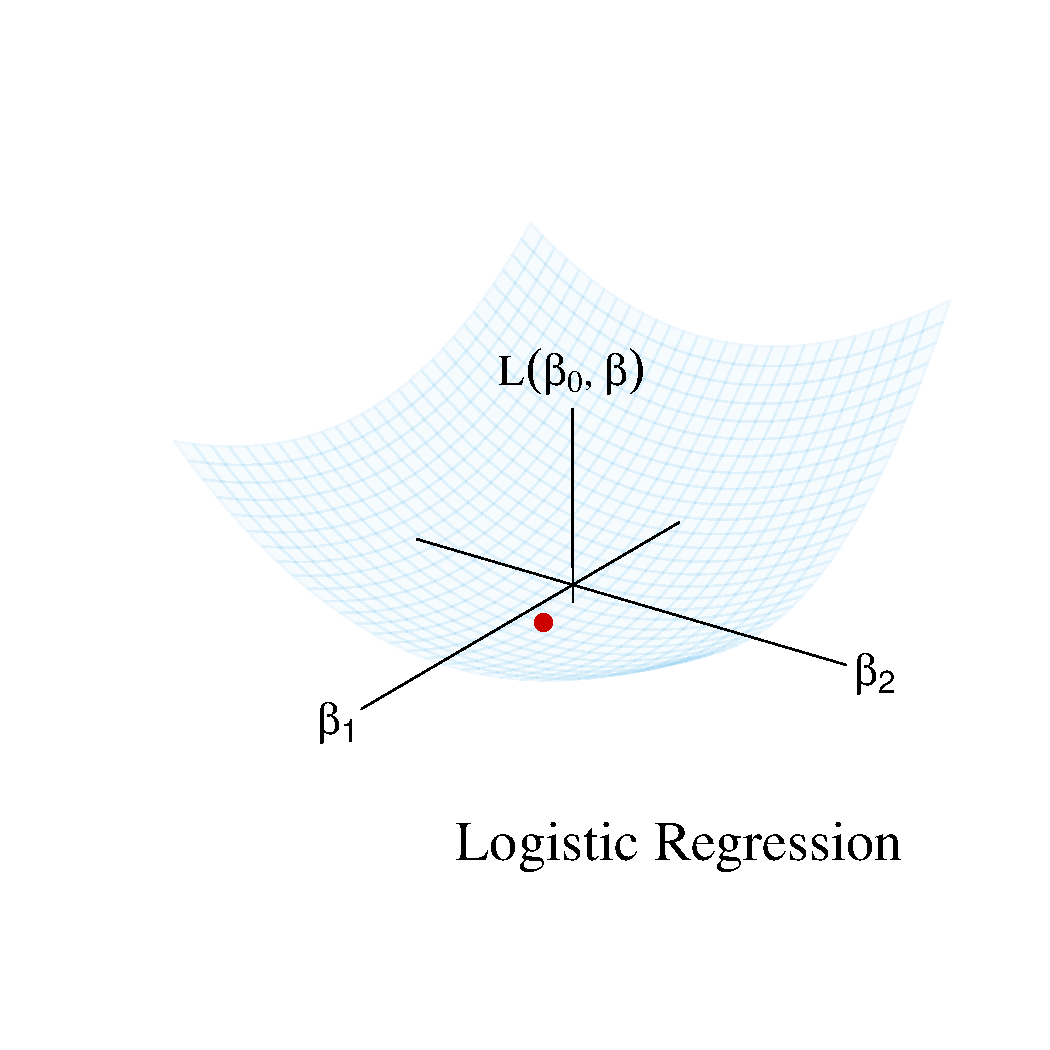
\includegraphics[trim = 50 50 0 50, clip, width = 0.33\textwidth]{min_nll.pdf}
    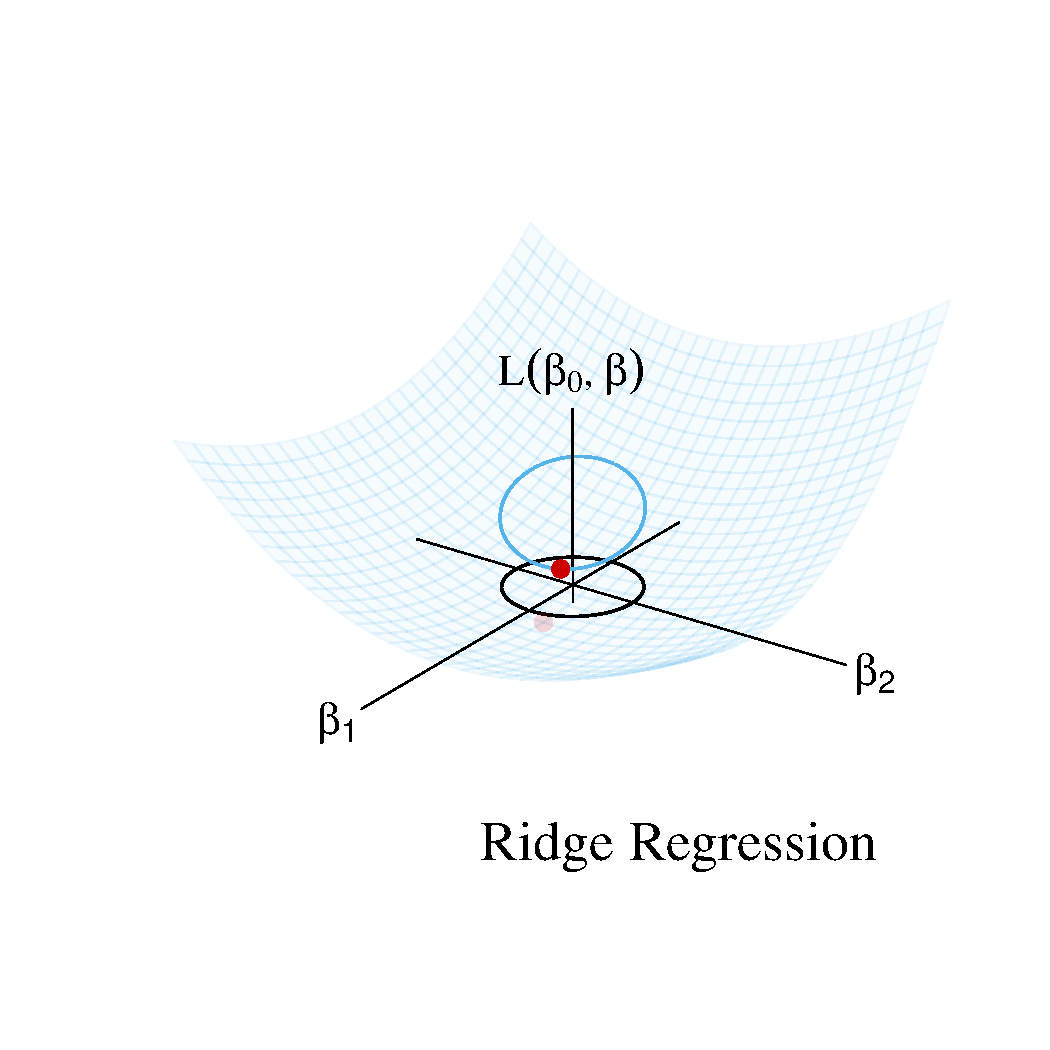
\includegraphics[trim = 50 50 0 50, clip, width = 0.475\textwidth]{min_ridge.pdf}
    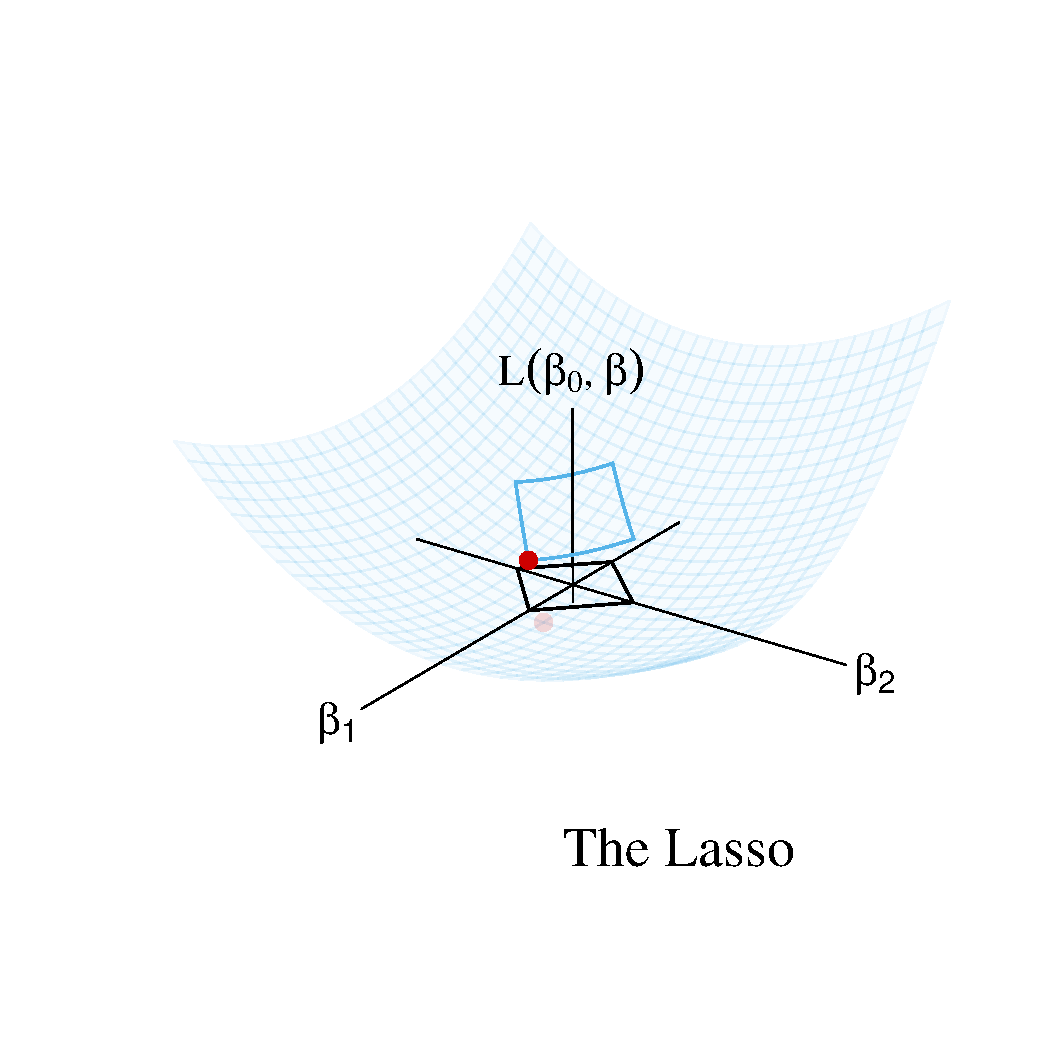
\includegraphics[trim = 50 50 0 50, clip, width = 0.475\textwidth]{min_lasso.pdf}
\end{figure}

Here is a special case of $L(\beta_0, \bm{\beta})$ with two predictors, so $\bm{\beta} = (\beta_1,\beta_2)$ (and a fixed value of $\beta_0$).
\begin{itemize}
    \item For two predictors, $\| \bm{\beta} \|_2^2 = \beta_1^2 + \beta_2^2$ and $\| \bm{\beta} \|_1 = |\beta_1| + |\beta_2|$.
    \item The new location of the minimum lies along the contour lines of the penalty! 
    \item Here, we can see that the lasso sets $\beta_1 = 0$. This happens a lot due to the sharp corners of the $\ell_1$ norm penalty.
\end{itemize}
    
\end{frame}

\begin{frame}{The Elastic Net}

Both ridge regression and the lasso have their own benefits and drawbacks. 
\begin{itemize}
    \item By combining the two, we can get the best of both worlds!
\end{itemize} \mys

The \textit{elastic net} minimizes 
\begin{align}
    \label{enet}
    Q(\beta_0, \bm{\beta}) = L(\beta_0, \bm{\beta})
    + \lambda \Big[ \alpha \| \bm{\beta} \|_{1} + \frac{1 - \alpha}{2} \|\bm{\beta}\|_{2}^{2} \Big].
\end{align} \mysa

The elastic net is a generalization of ridge regression and the lasso.
\begin{itemize}
    \item The mixing parameter $\alpha \in [0,1]$ controls how much of each type of penalty is imposed on the model.
    \item $\alpha = 0 \to$ ridge regression.
    \item $\alpha = 1 \to$ the lasso.
\end{itemize} \mys

The elastic net (including ridge regression and the lasso) can be implemented efficiently using the \texttt{glmnet} package in \texttt{R}. %\Laughey[1.5][yellow][pink] 
    
\end{frame}

\begin{frame}{\color{white} Contour Plots}

\begin{center}
    \centering
    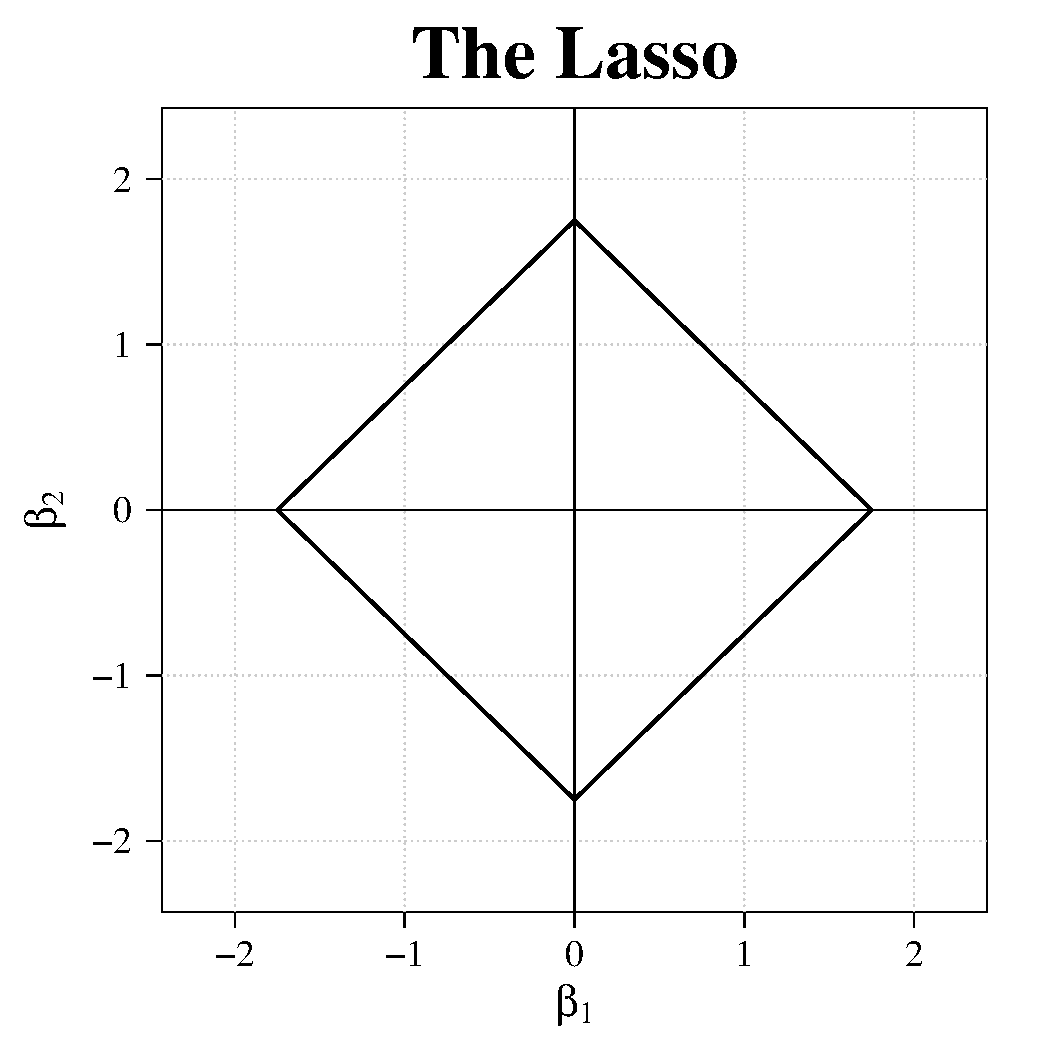
\includegraphics[width = 0.33\textwidth]{cont_lasso.pdf}
    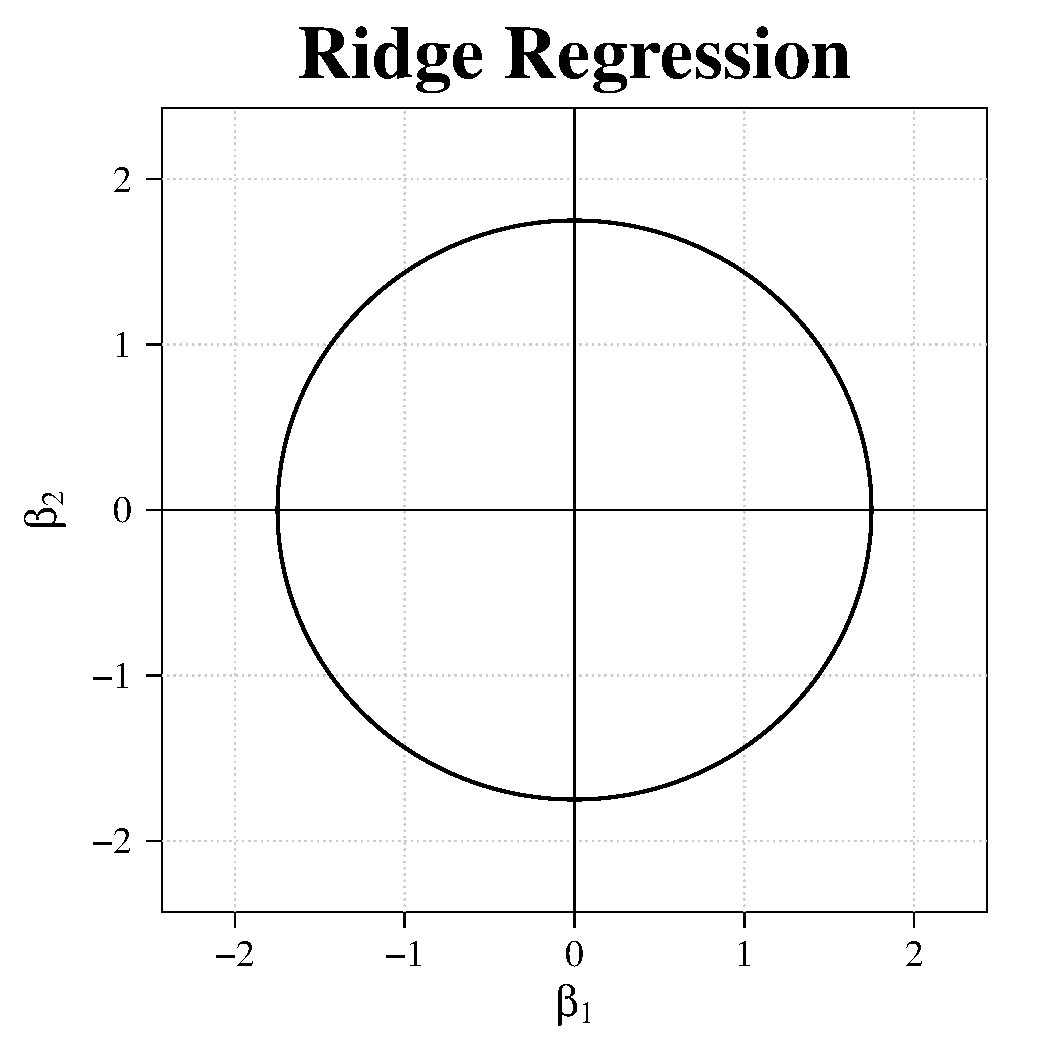
\includegraphics[width = 0.33\textwidth]{cont_ridge.pdf}
    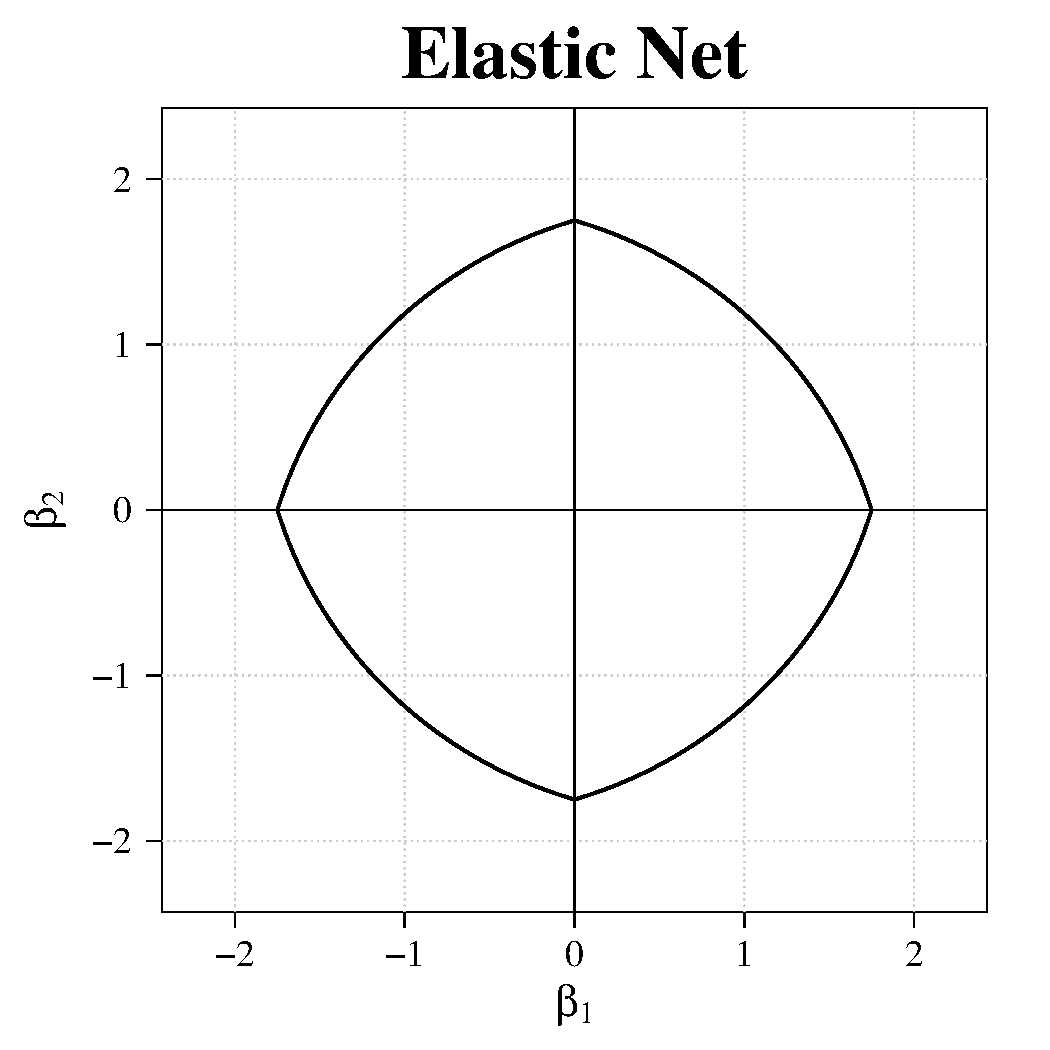
\includegraphics[width = 0.33\textwidth]{cont_enet.pdf}
    %\animategraphics[autoplay, loop, width = 0.33\textwidth]{30}{enet_ani_merged}{}{}
\end{center}

The \textit{shape} of the penalty can give some idea of the type of shrinkage imposed on the model.
\begin{itemize}
    \item Sharp corners $\to$ sparsity! \Laughey[1.5][yellow][pink]
    \item Round corners $\to$ only shrinkage!
\end{itemize}
    
\end{frame}


\begin{frame}[noframenumbering]{\color{white} Contour plots}

\begin{center}
    \centering
    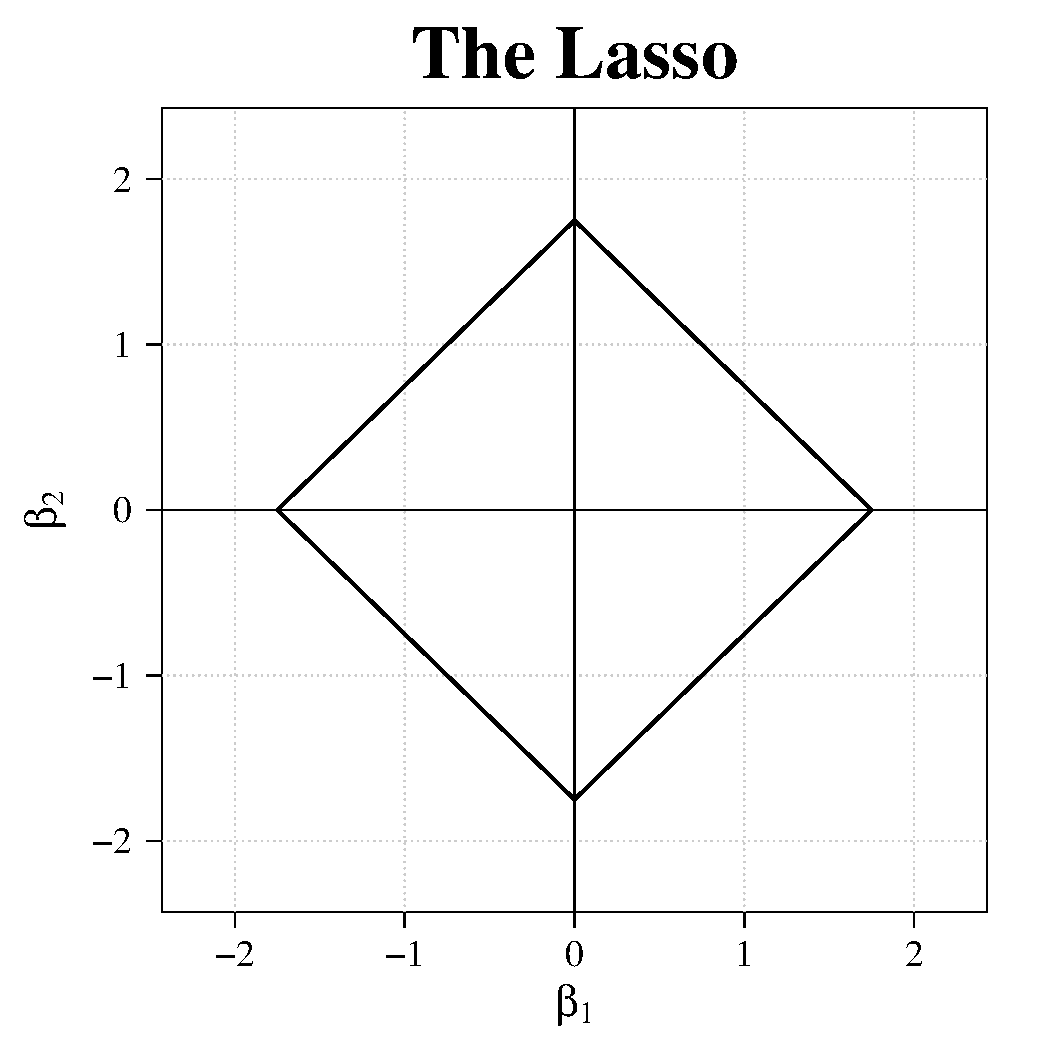
\includegraphics[width = 0.33\textwidth]{cont_lasso.pdf}
    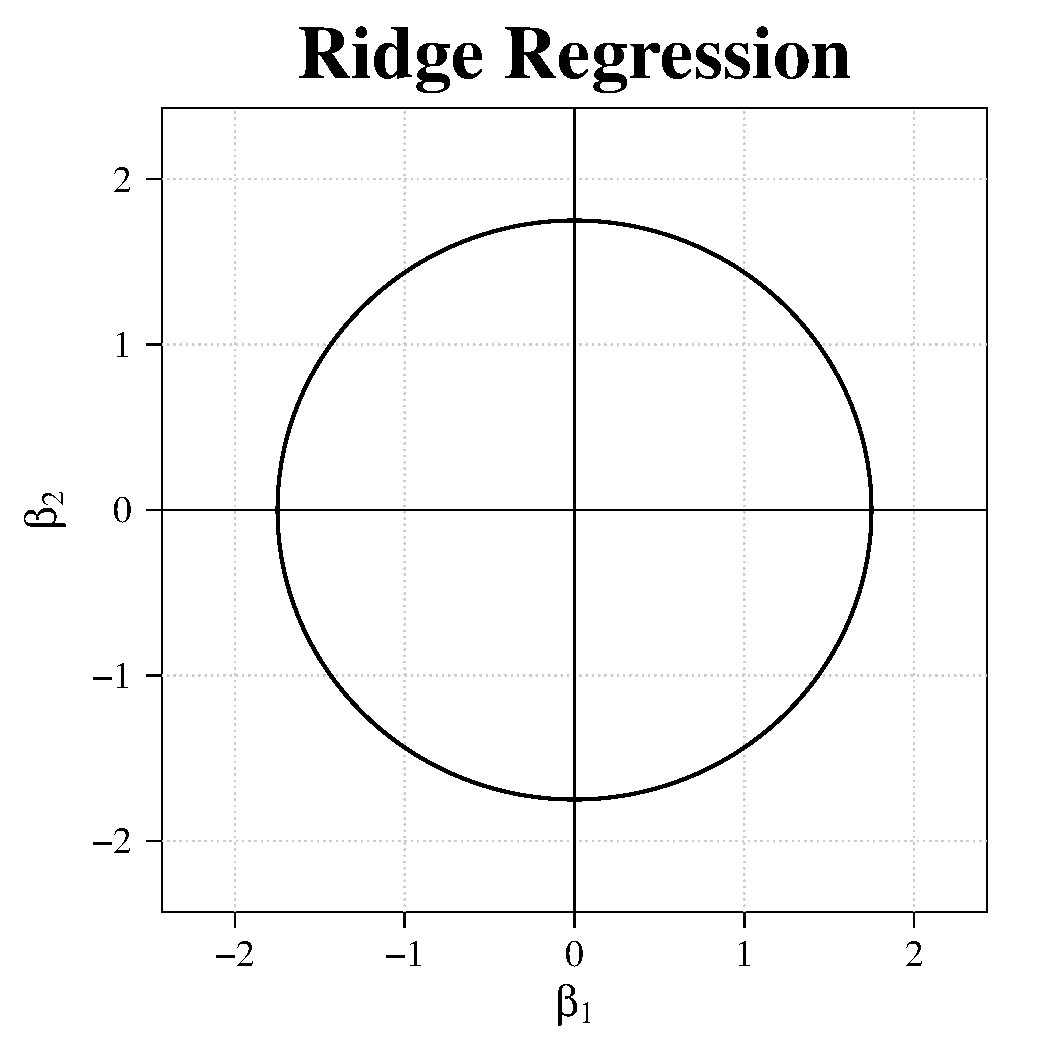
\includegraphics[width = 0.33\textwidth]{cont_ridge.pdf}
    %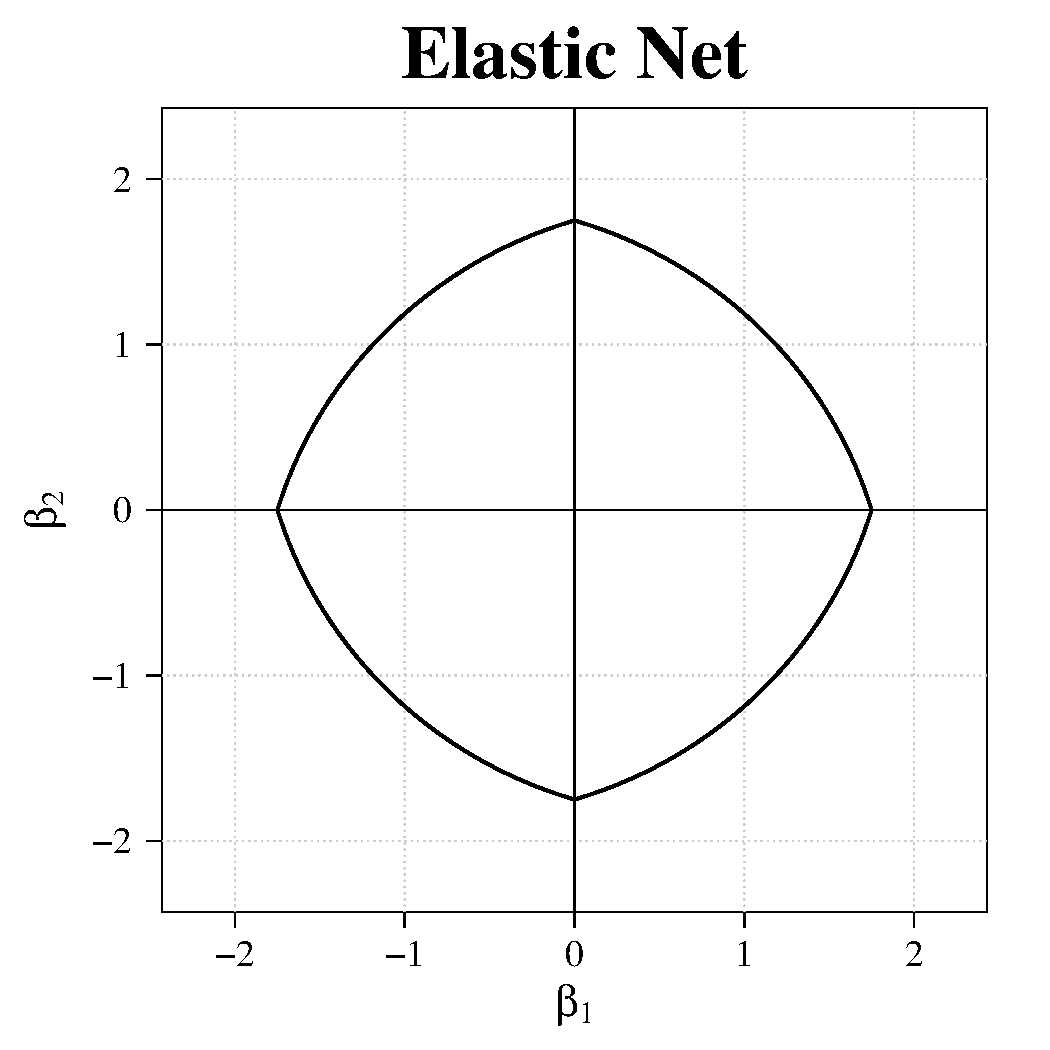
\includegraphics[width = 0.33\textwidth]{cont_enet.pdf}
    \animategraphics[autoplay, loop, width = 0.33\textwidth]{30}{enet_ani_merged}{}{}
\end{center}
The \textit{shape} of the penalty can give some idea of the type of shrinkage imposed on the model.
\begin{itemize}
    \item Sharp corners $\to$ sparsity! \Laughey[1.5][yellow][pink]
    \item Round corners $\to$ only shrinkage!
\end{itemize}
    
\end{frame}

\begin{frame}{The Group Setting}

If the predictors belong to pre-defined groups, basic regularization might perform poorly.
\begin{itemize}
    \item e.g. The genes of the colon data set belong to gene pathways.
    \item In truth, it might be that only some of these pathways affect the response.
    \item However, the lasso might select genes that are not in this pathway! %\Sadey[1.5][yellow]
\end{itemize} \mys

We assume that the predictors belong to $K$ \textit{non-overlapping} groups.
\begin{itemize}
    \item Let $S_k$ denote the number of predictors in the $k$th group.
    \item Let $\mathbf{X}_k \in \mathbb{R}^{N \times S_k}$ be the sub-matrix corresponding to the $k$th group.
    \item Let $\bm{\beta}_k \in \mathbb{R}^{S_k}$ be the sub-vector corresponding to the $k$th group.
\end{itemize} \mys

We can exploit this group structure to improve our model's prediction accuracy and interpretability.
    
\end{frame}

\begin{frame}{\color{white} The Group Lasso}

The \textit{group lasso} minimizes 
\begin{align}
    \label{grouplasso}
    Q(\beta_0, \bm{\beta}) = L(\beta_0, \bm{\beta}) + \sum_{k=1}^K \sqrt{S_k} \| \mathbf{X}_k \bm{\beta}_k \|_2.
\end{align} \mysa

Instead of selecting significant predictors, the group lasso selects significant \textit{groups}.
\begin{itemize}
    \item e.g. In the colon data set, only 3 of the 9 total groups were significant.
    \item The penalty acts like the lasso to coefficients in \textit{different} groups, while acting like ridge regression to coefficients in \textit{the same} group.
\end{itemize} \mys

However, this is one of the major drawbacks of the group lasso.
\begin{itemize}
    \item If a group is significant, \textit{all of the predictors will be in the final model}.
    \item In truth, it may be that only some predictors from the significant groups affect the response. %\Sadey[1.5][yellow]
    \item The group lasso cannot perform \textit{bi-variate selection}.
\end{itemize}
    
\end{frame}

\begin{frame}{Sparse Group Lasso}

One method that can select bi-variate selection is the \textit{sparse group lasso}. It minimizes 
\begin{align}
    \label{sparsegrouoplasso}
    Q(\beta_0, \bm{\beta}) = L(\beta_0, \bm{\beta}) + \lambda \left[ \alpha \| \bm{\beta} \|_1 + (1 - \alpha) \sum_{k=1}^K \sqrt{S_k}  \| \bm{\beta}_k \|_2 \right].
\end{align} \mysa

Similar to the elastic net, this is a generalization of the lasso and the group lasso.
\begin{itemize}
    \item $\alpha = 0 \to$ the group lasso.
    \item $\alpha = 1 \to$ the lasso.
    \item The penalty acts like the lasso to coefficients in \textit{different} groups, while acting like the elastic net to coefficients in \textit{the same} group.
\end{itemize} \mys

In theory: \Laughey[1.5][yellow][pink] ~In practice: \Vomey[1.5][yellow][Green]
\begin{itemize}
    \item The group lasso can be efficiently implemented using the \texttt{grpreg} package in \texttt{R}.
    \item The sparse group lasso is implemented by the \texttt{SGL} package in \texttt{R}, which is not efficient and extremely unstable, i.e. it caused \texttt{R} to crash most of the time.
    \item This actually was a huge issue for our research.
\end{itemize}
    
\end{frame}

\begin{frame}{Contour Plots}

\begin{center}
    %\centering
    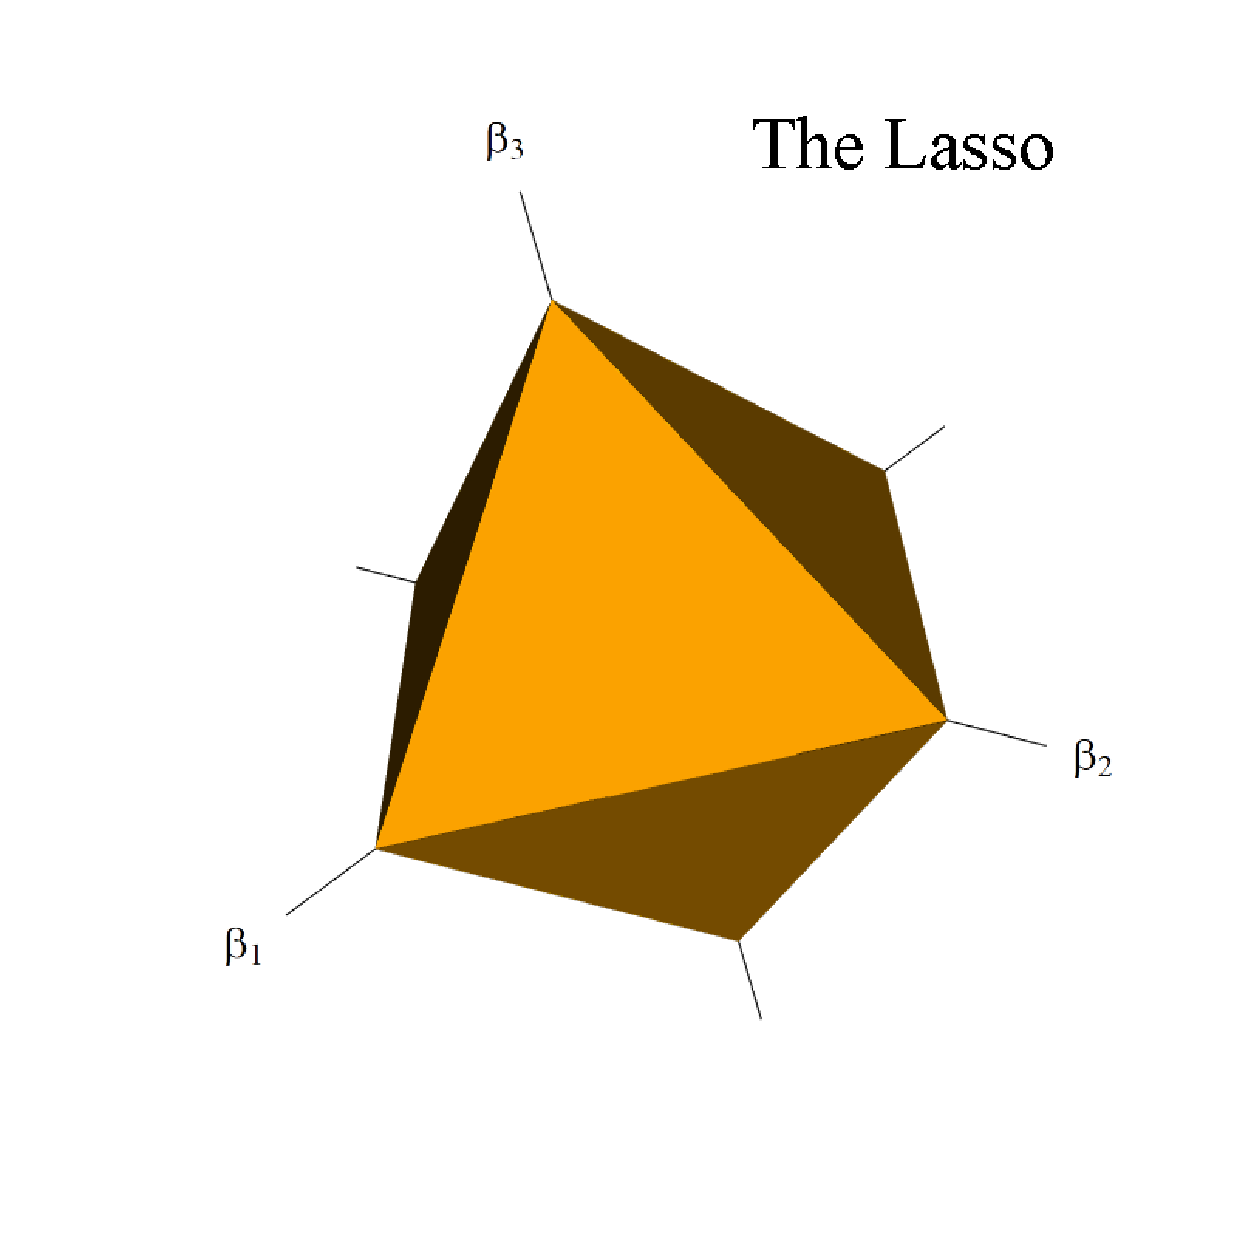
\includegraphics[width = 0.33\textwidth]{3D_cont_lasso.pdf}
    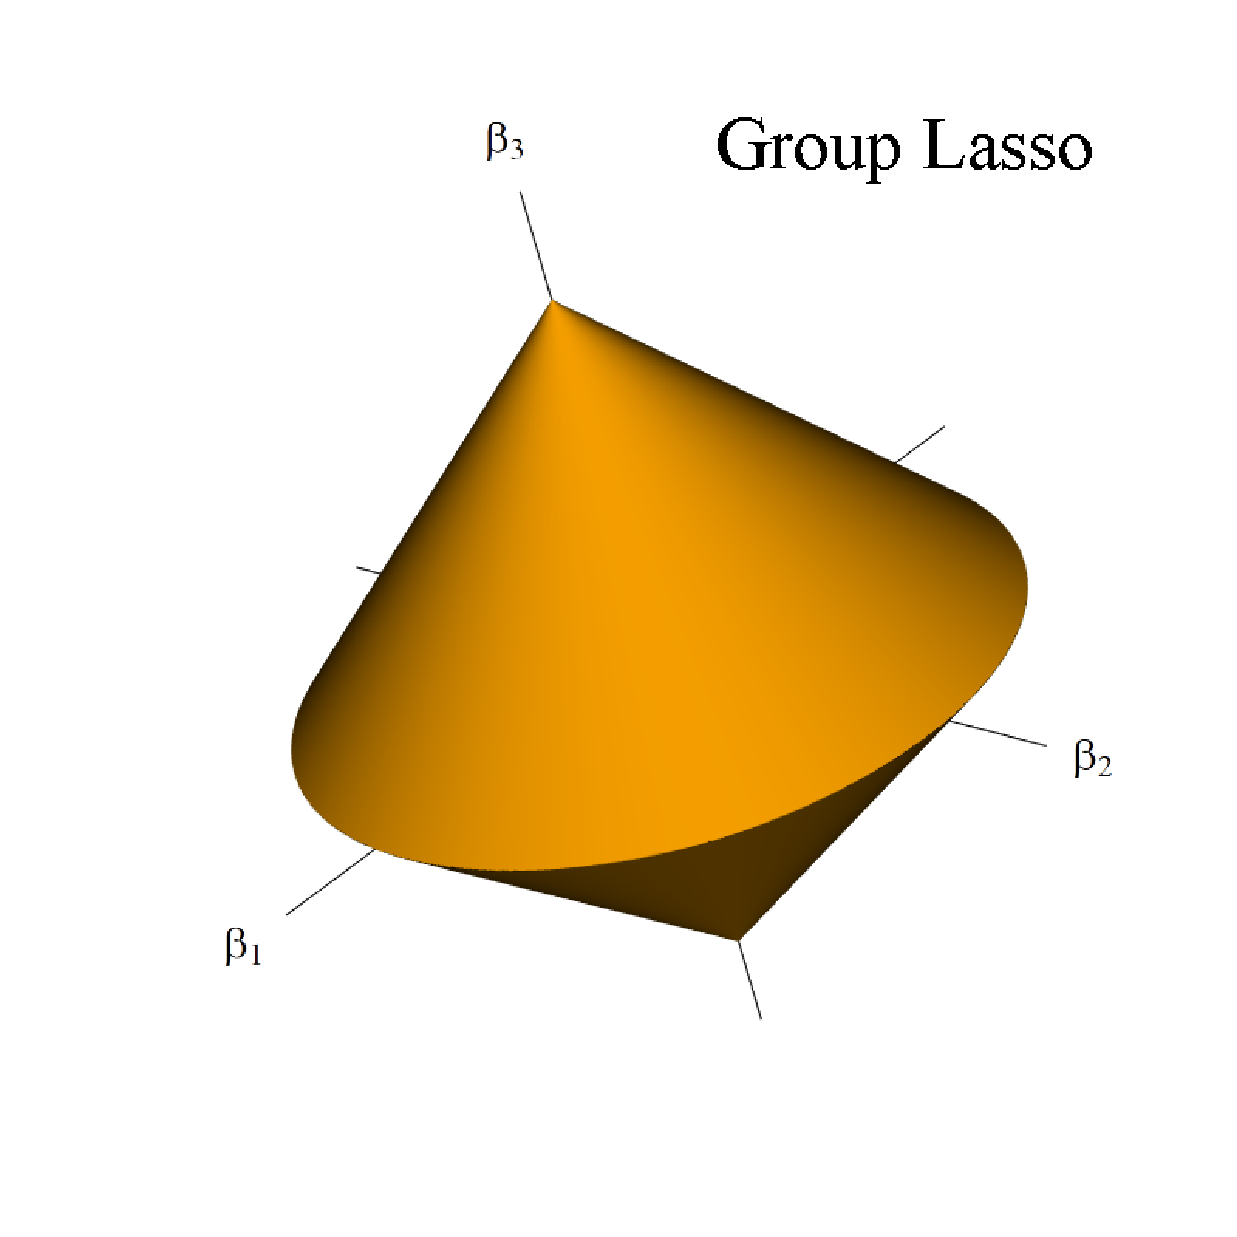
\includegraphics[width = 0.33\textwidth]{3D_cont_glasso.pdf}
    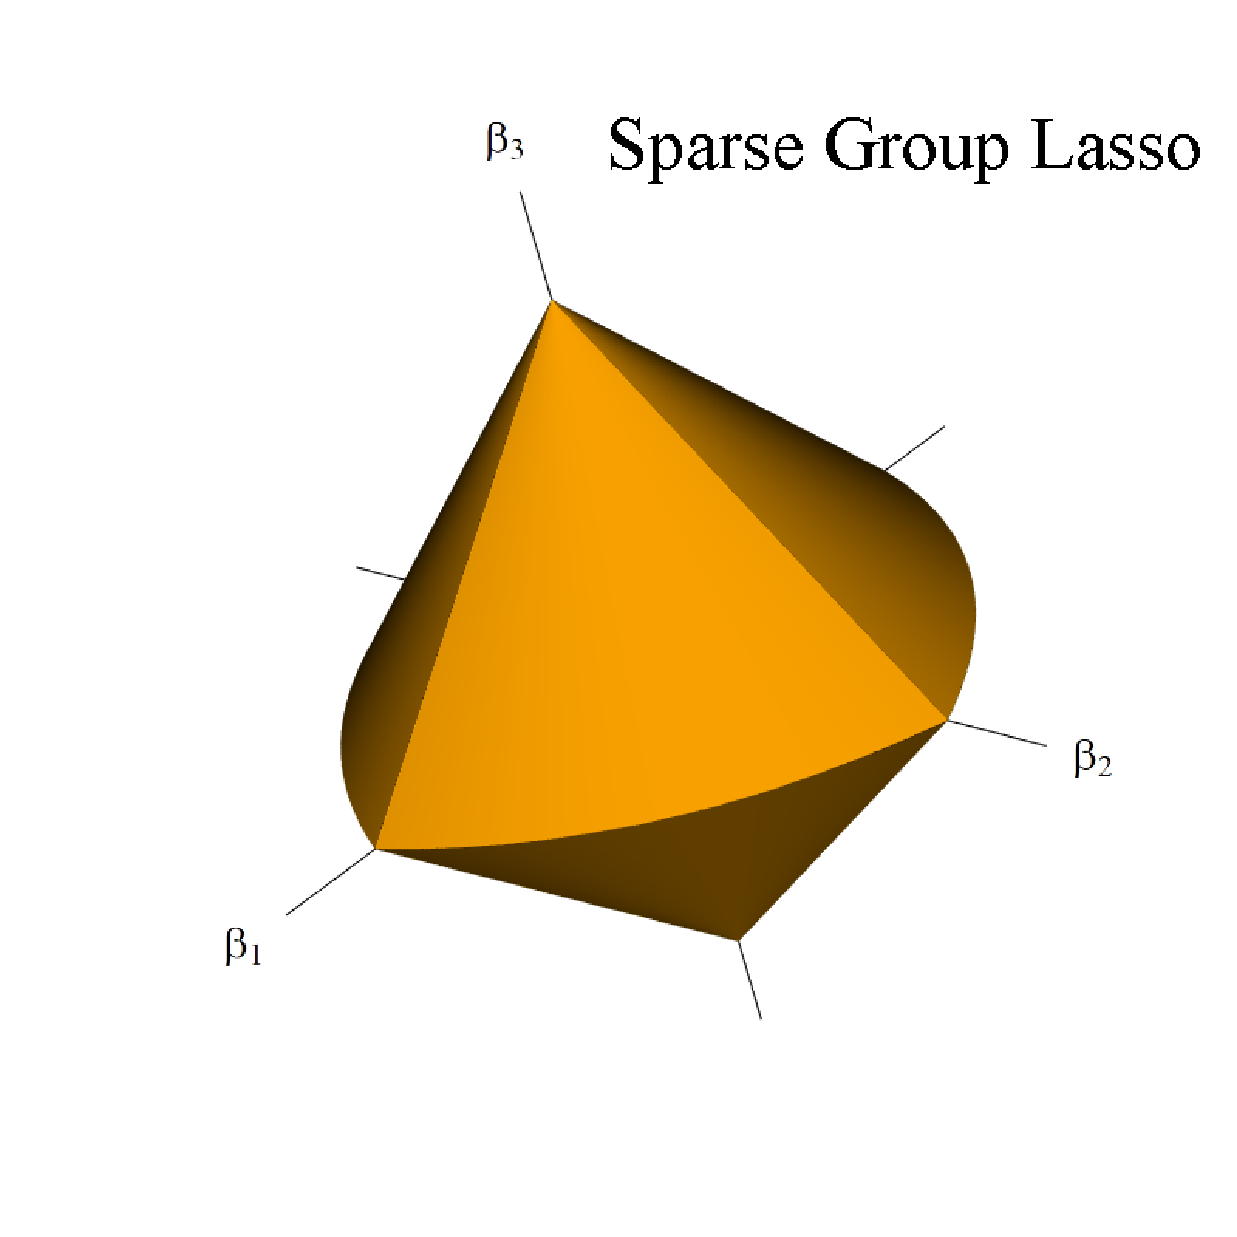
\includegraphics[width = 0.33\textwidth]{3D_cont_sglasso.pdf}
    %\animategraphics[autoplay, loop, width = 0.33\textwidth]{30}{enet_ani_merged}{}{}
\end{center}

Here is a special case with three predictors, grouped so that $\bm{\beta_1} = (\beta_1, \beta_2)$ and $\bm{\beta}_2 = \beta_3$.
\begin{itemize}
    \item Sharp points between coefficients not in the same group (e.g. $\beta_1$ and $\beta_3$) $\to$ sparsity at the group level.
    \item Round points between coefficients in the same group ($\beta_1$ and $\beta_2$) $\to$ only shrinkage within the group.
    \item Sparse group lasso is a compromise.
\end{itemize}
    
\end{frame}

\begin{frame}{Composite Minimax Concave Penalty}

Another method that can perform bi-variate selection is the \textit{composite minimax concave penalty} (``cMCP''). It minimizes
\begin{align}
    \label{cMCP}
    Q(\beta_0, \bm{\beta}) = L(\beta_0, \bm{\beta}) + \sum_{k=1}^K f_{\lambda, \Gamma_k} \left( \sum_{s=1}^{S_k} f_{\lambda, \gamma}(|\beta_{k,s}|) \right),
\end{align}
where $f_{\lambda, \gamma}(\cdot)$ is given by
\begin{align}
    \label{MCPpenalty}
    f_{\lambda, \gamma}(\phi) = \begin{cases}
        \lambda \phi - \frac{\phi^2}{2 \gamma}, & \text{if } \phi \le \gamma \lambda \\
        \frac{1}{2} \gamma \lambda^2, & \text{if } \phi > \gamma \lambda
    \end{cases}.
\end{align} \mys

Explaining the theory would take too long! \Sadey[1.5][yellow]
\begin{itemize}
    \item Just know that it performs bi-variate selection.
    \item It can also be efficiently implemented using the \texttt{grpreg} package in \texttt{R}.
    \item These reasons are why we chose cMCP.
\end{itemize}
    
\end{frame}

\begin{frame}{\color{white} Principal Component Analysis}

The \textit{singular value decomposition} of the data matrix $\mathbf{X}$ is given by 
\begin{align}
    \label{SVD}
    \mathbf{X} = \mathbf{U} \mathbf{D} \mathbf{V}^T,
\end{align}
where 
\begin{itemize}
    \item $m = \mathrm{rank}(\mathbf{X})$.
    \item $\bm{d} = (d_1, \ldots, d_m)$ are the singular values, and $\mathbf{D} = \mathrm{diag}(d_1, \ldots, d_m)$.
    \item The columns of $\mathbf{V} \in \mathbb{R}^{P \times m}$ are the \textit{principal axes}.
    \item The columns of $\mathbf{U} \mathbf{D} \in \mathbb{R}^{N \times m}$ are the \textit{principal components}.
\end{itemize} \mys

The principal axes $\bm{v}_1, \ldots, \bm{v}_m$ are the directions in which the data vary the most.
\begin{itemize}
    \item It can be shown that ridge regression slightly biases $\bm{\beta}$ in the direction of the leading principal axis $\bm{v}_1$.
    \item By strongly biasing $\bm{\beta}$ in the direction of $\bm{v}_1$, we can further improve prediction accuracy.
\end{itemize}
    
\end{frame}

\begin{frame}{\color{white} Principal Components Lasso}

\textit{Principal components lasso} (``pcLasso'') minimizes
\begin{align}
    \label{pclasso}
    Q(\beta_0, \bm{\beta}) = L(\beta_0, \bm{\beta}) + \lambda \| \bm{\beta} \|_1 + \frac{\theta}{2} \bm{\beta}^T \Big( \mathbf{V} \mathbf{D}_{d_1^2 - d_j^2} \mathbf{V}^T \Big) \bm{\beta},
\end{align}
where 
\begin{align}
    \label{pclassopenaltymatrix}
    \mathbf{D}_{d_1^2 - d_j^2} = \mathrm{diag}(d_1^2 - d_1^2, d_1^2 - d_2^2, \ldots, d_1^2 - d_m^2).
\end{align} \mys

This penalty corresponds to more aggressive bias in the direction of $\bm{v}_1$.
\begin{itemize}
    \item The parameter $\theta$ controls how strong this bias is.
    \item The $\ell_1$ norm penalty allows pcLasso to induce sparsity in the model.
\end{itemize} \mys

pcLasso can also be extended to regularize grouped predictors.
\begin{itemize}
    \item In this case, each group vector $\bm{\beta}_k$ is biased in the direction of that group's leading principal axis.
    \item Both grouped and non-grouped pcLasso can be efficiently implemented by the \texttt{pcLasso} package in \texttt{R}.
\end{itemize}
    
\end{frame}

\begin{frame}{Contour plots}

\begin{center}
    \centering
    \textcolor{white}{\frame{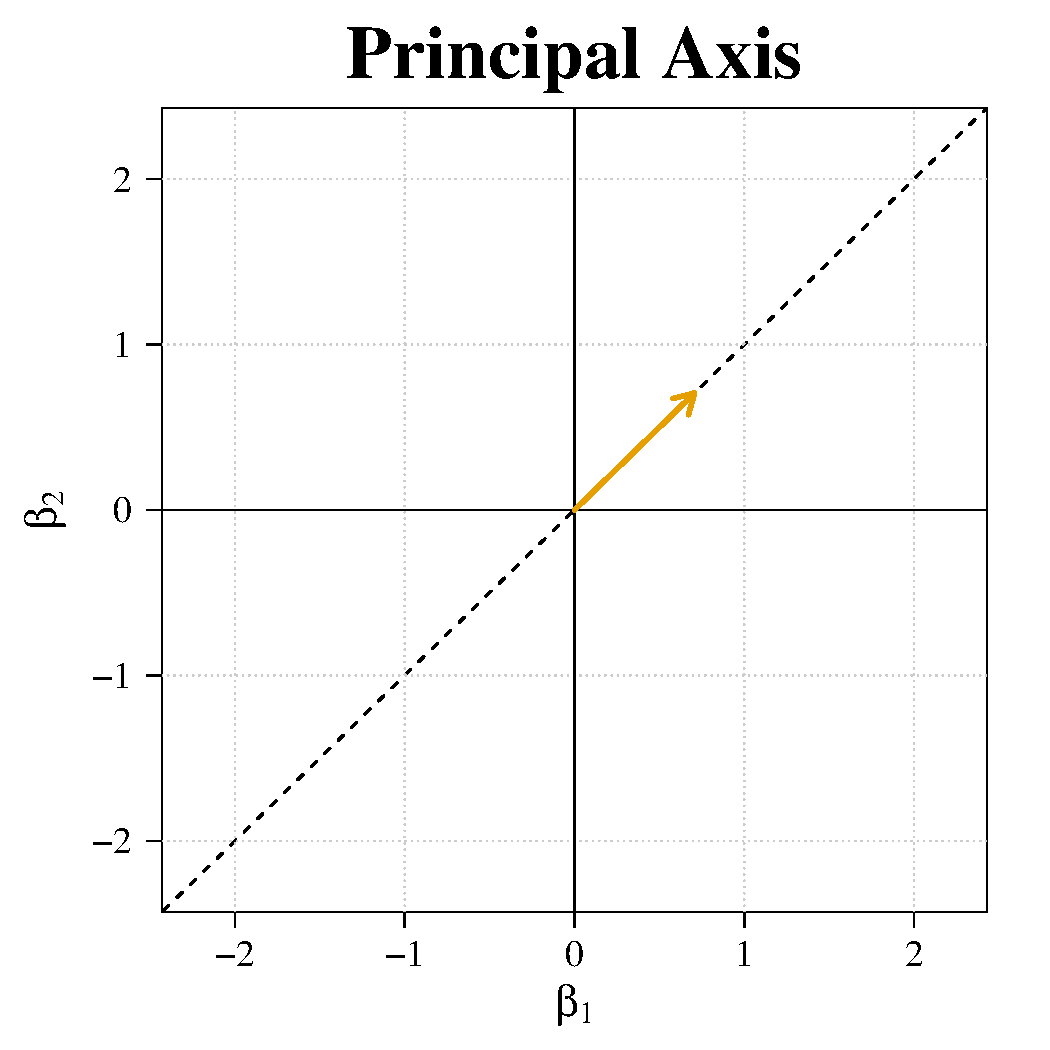
\includegraphics[width = 0.475\textwidth]{principal_axis.pdf}}}
    \textcolor{white}{\frame{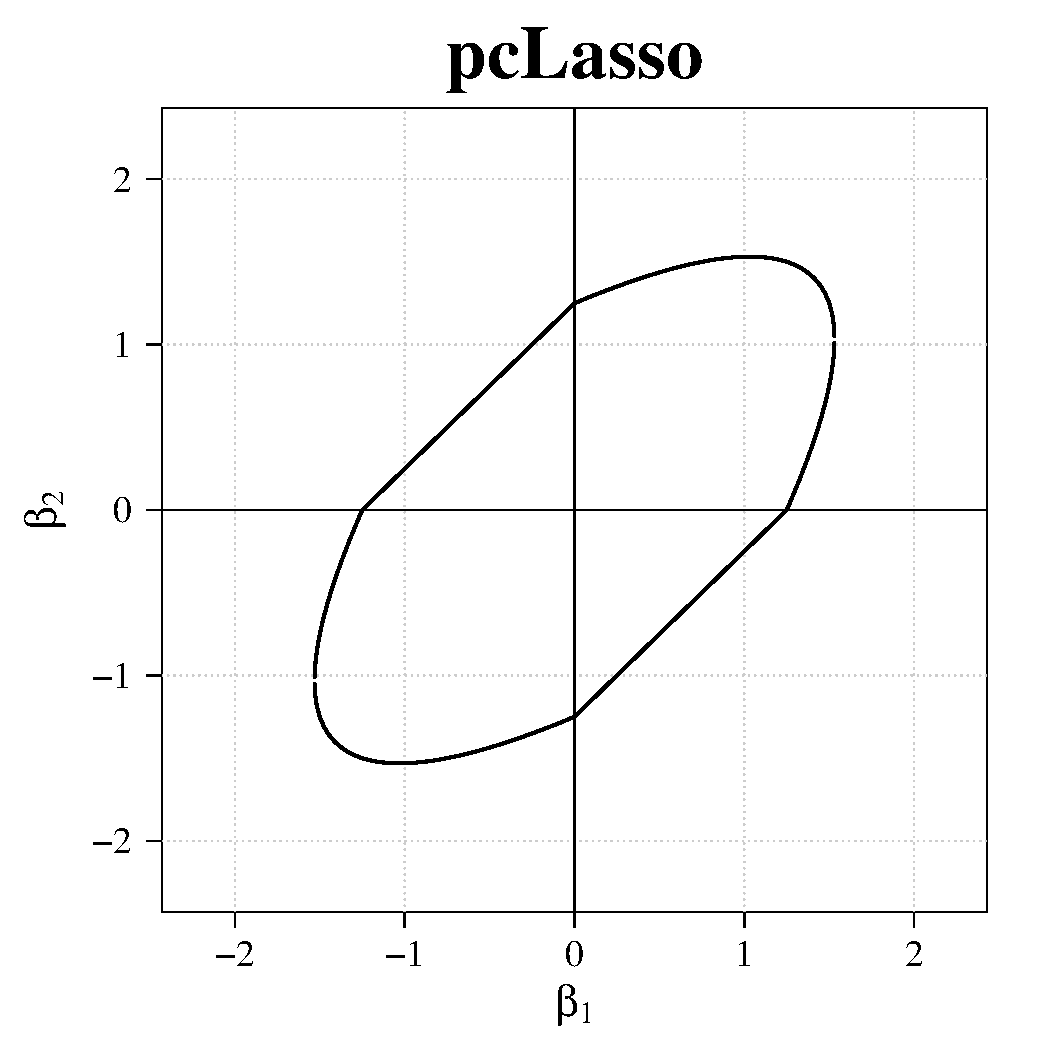
\includegraphics[width = 0.475\textwidth]{cont_pcl.pdf}}}
\end{center}

In a special case of two positively-correlated predictors, the leading principal axis is $\bm{v}_1 = (1/\sqrt{2}, 1/\sqrt{2})$.
\begin{itemize}
    \item As $\theta \to \infty$, the contour lines become a line segment in the direction of $\bm{v}_1$.
    \item As $\theta \to 0$, the contour line becomes more similar to the lasso.
\end{itemize}
    
\end{frame}

\begin{frame}[noframenumbering]{Contour plots}

\begin{center}
    \centering
    \textcolor{white}{\frame{\animategraphics[autoplay, loop, width = 0.475\textwidth]{30}{cont_pcl_grow}{}{}}}
    \textcolor{white}{\frame{\animategraphics[autoplay, loop, width = 0.475\textwidth]{30}{cont_pcl_shrink}{}{}}}
\end{center}

In a special case of two positively-correlated predictors, the leading principal axis is $\bm{v}_1 = (1/\sqrt{2}, 1/\sqrt{2})$.
\begin{itemize}
    \item As $\theta \to \infty$, the contour lines become a line segment in the direction of $\bm{v}_1$.
    \item As $\theta \to 0$, the contour line becomes more similar to the lasso.
\end{itemize}
    
\end{frame}

\begin{frame}{\color{white} Clustering}

\textit{Clustering} is an unsupervised learning method that splits the predictors up into different groups.
\begin{itemize}
    \item Predictors in the same group will be similar, while predictors in different groups will not.
    \item This is an unsupervised learning algorithm, since we are tying to get information about the data without a measurable response.
\end{itemize} \mys

The choice of how ``similarity'' is defined will greatly impact the resulting group structure. Two common choices:
\begin{enumerate}
    \item Euclidean distance.
    \item Correlation.
\end{enumerate} \mys

There are \textit{many} different clustering algorithms that could be used, so we decided to go with two common ones.
    
\end{frame}

\begin{frame}{$K$-means clustering}

\textit{$K$-means clustering} attempts to divide the predictors into $K$ non-overlapping groups.
\begin{itemize}
    \item Let $S_k$ be the number of predictors in the $k$th group.
    \item Let $\mathcal{C}_k$ denote the set containing all predictors in group $k$.
\end{itemize} \mys

The $K$ clusters are chosen to minimize the \textit{total within-cluster variation}, given by 
\begin{align}
    \label{totwithinclusvar}
    W_K = \sum_{k=1}^K \sum_{j \in \mathcal{C}_k} \| \mathbf{x}_j - \bar{\mathbf{x}}_k \|_2^2,
\end{align}
where $\mathbf{x}_j$ is the $j$th predictor and $\bar{\mathbf{x}}_k = \frac{1}{S_k} \sum_{j \in \mathcal{C}_k} \mathbf{x}_j$ is the $k$th group centroid. \mys

The main drawback to $K$-means clustering is that we need to know the number of clusters $K$ \textit{beforehand}.
\begin{itemize}
    \item We have no inference of the data, so instead we want some automated way to choose the ``optimal'' number of clusters.
    \item One way to do this is the GAP statistic -- no details here.
\end{itemize}
    
\end{frame}

\begin{frame}{$\ldots$}

\begin{figure}
    \centering
    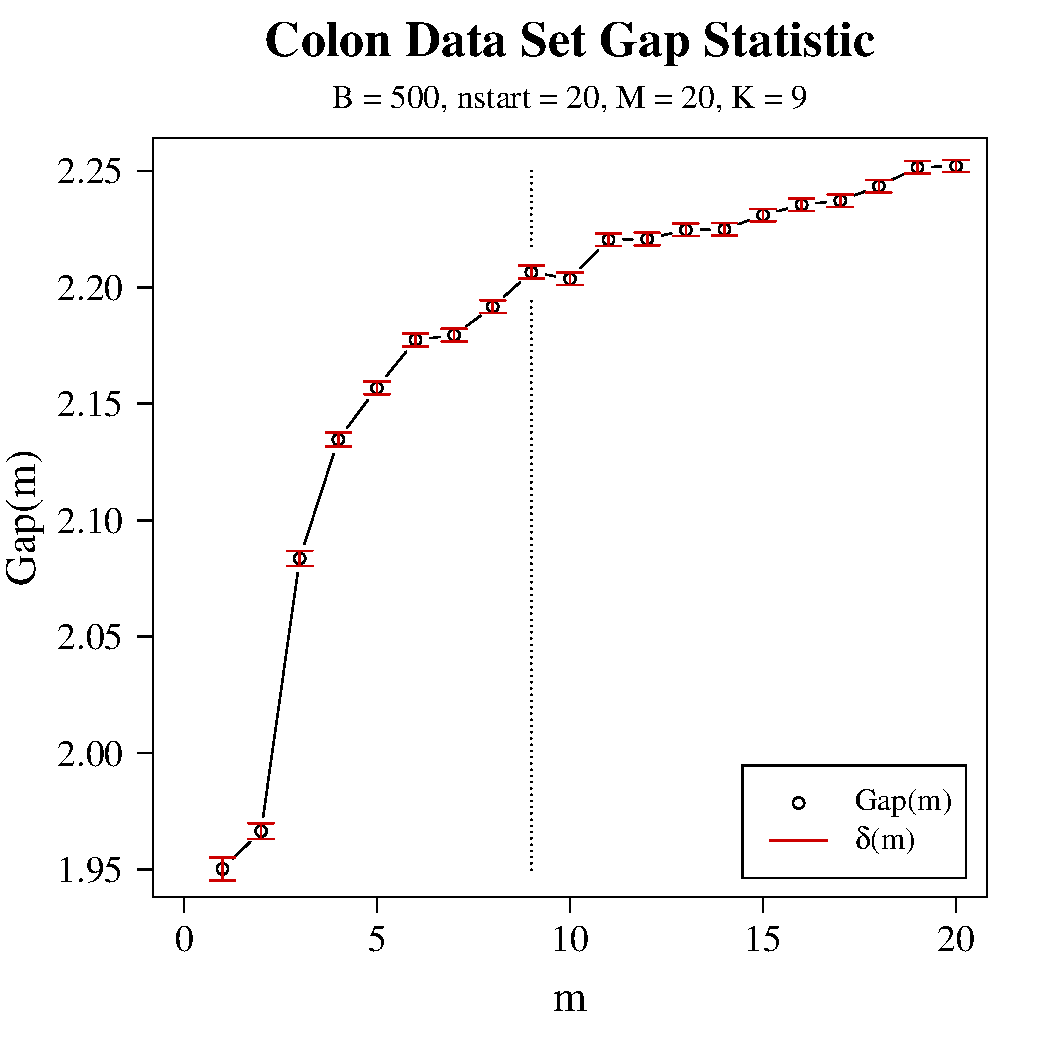
\includegraphics[width = 0.475\textwidth]{colon_gap_stat.pdf}
    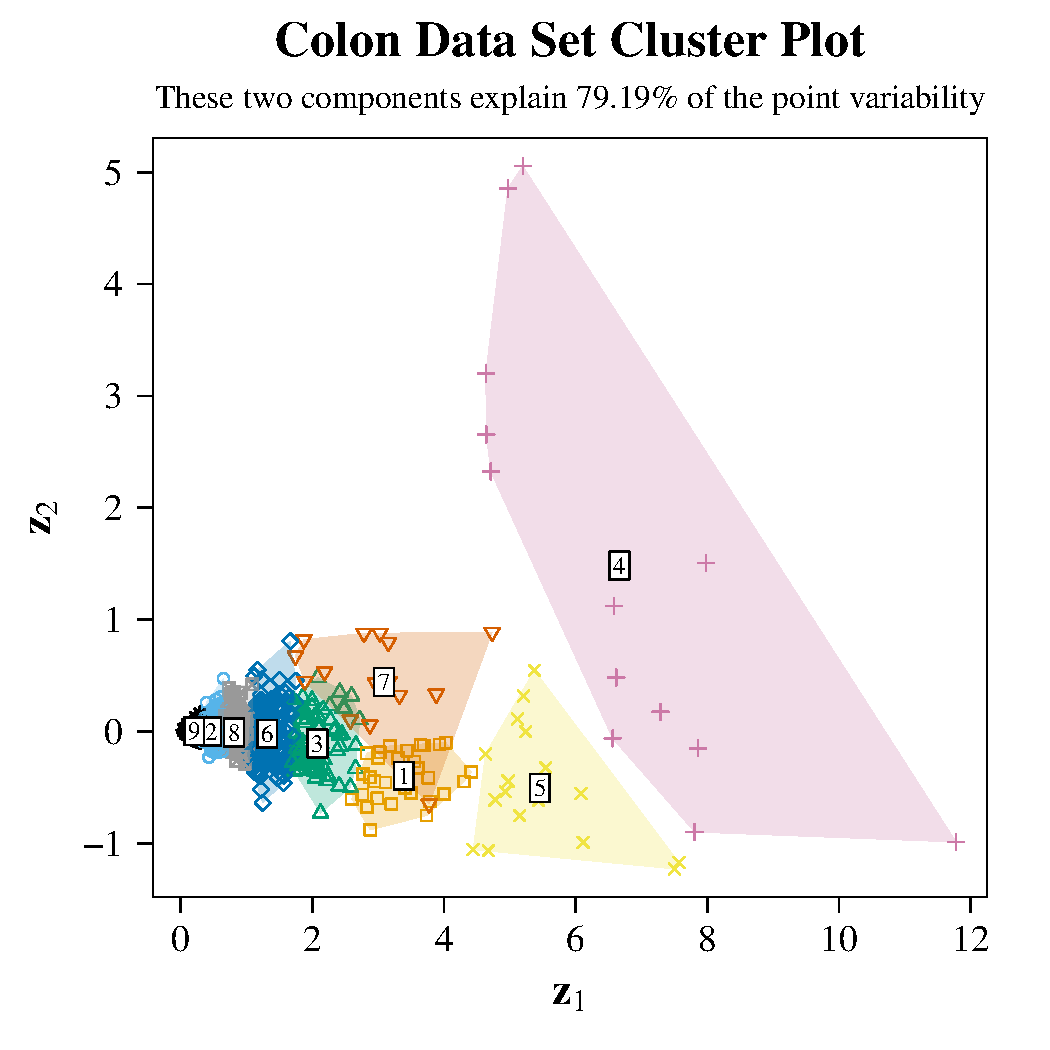
\includegraphics[width = 0.475\textwidth]{colon_clus_plot.pdf}
\end{figure}

Here is the result of using $K$-means clustering on the colon data set.
\begin{itemize}
    \item The predictors are plotted against the first two columns of $\mathbf{Z} = \mathbf{V} \mathbf{D}$.
    \item The GAP statistic chooses $K=9$ as the optimal amount of clusters.
    \item Are these clusters really well-separated? %\Tongey[1.5][yellow][pink]
\end{itemize}
    
\end{frame}

\begin{frame}{\color{white} Hierarchical clustering}

\begin{figure}
    \centering
    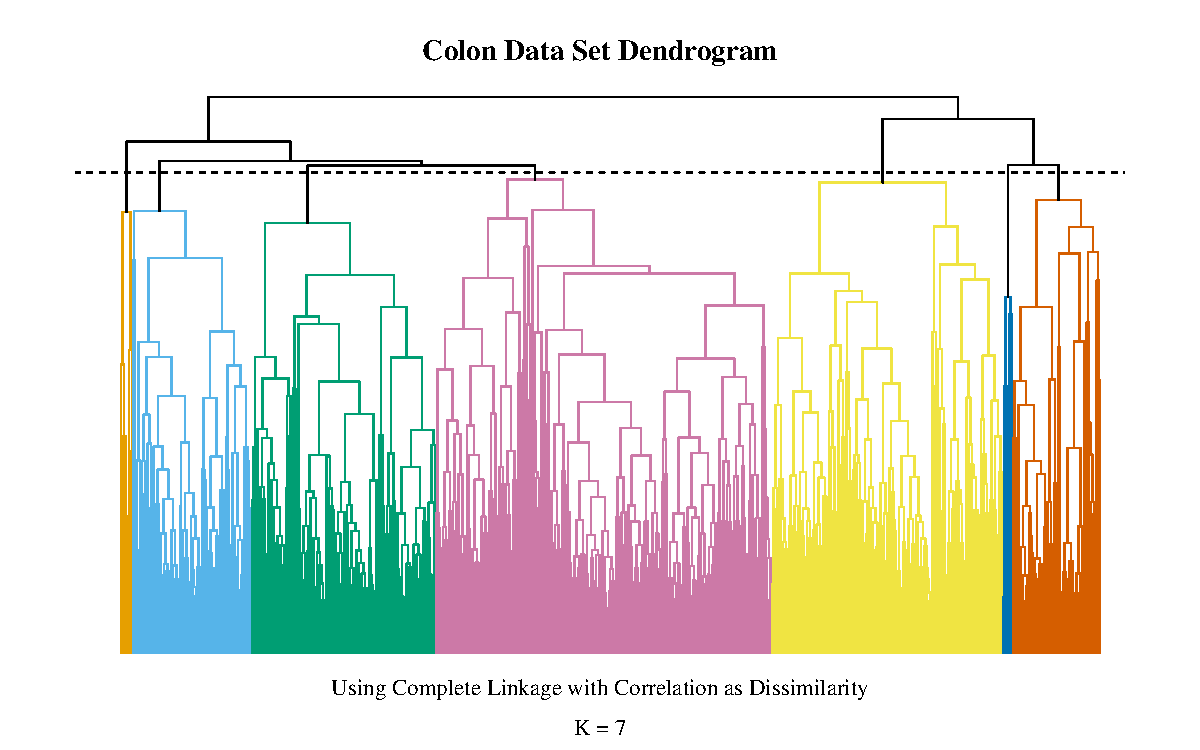
\includegraphics[width = 0.9\textwidth]{colon_den.pdf}
\end{figure}

Hierarchical clustering makes nested clusters (here it is based off of correlation).
\begin{itemize}
    %\item Tough to explain simply. %\Sadey[1.5][yellow]
    \item This clustering structure is presented in a \textit{dendrogram}.
    \item Here is the result of using hierarchical clustering on the colon data set.
    \item \textit{We} choose $K = 7$ as the optimal number of clusters.
\end{itemize}
    
\end{frame}

\begin{frame}{\color{white} Real-world examples}

For our report, we used two real-world data sets:
\begin{enumerate}
    \item The colon data set, $N = 62$, $P = 2000$ (we will focus on this one).
    \item The leukemia data set, $N = 72$, $P = 7128$.
\end{enumerate} \mys

We tested various models in the three following situations:
\begin{enumerate}
    \item The predictors were not clustered
    \item The predictors were clustered using $K$-means clustering
    \item The predictors were clustered using hierarchical clustering
\end{enumerate} \mys

Without clustering, we tested the lasso, the elastic net, and pcLasso. \mys

With both clustering methods, we tested the group lasso, the sparse group lasso, cMCP, and pcLasso. \mys

We randomly split the data in half, creating a training set and a test set.
\begin{itemize}
    \item The models were fit on the training set using 10-fold cross-validation. 
    \item The models were then evaluated on the test set. 
\end{itemize}
    
\end{frame}

\begin{frame}{Results}

\begin{center}
    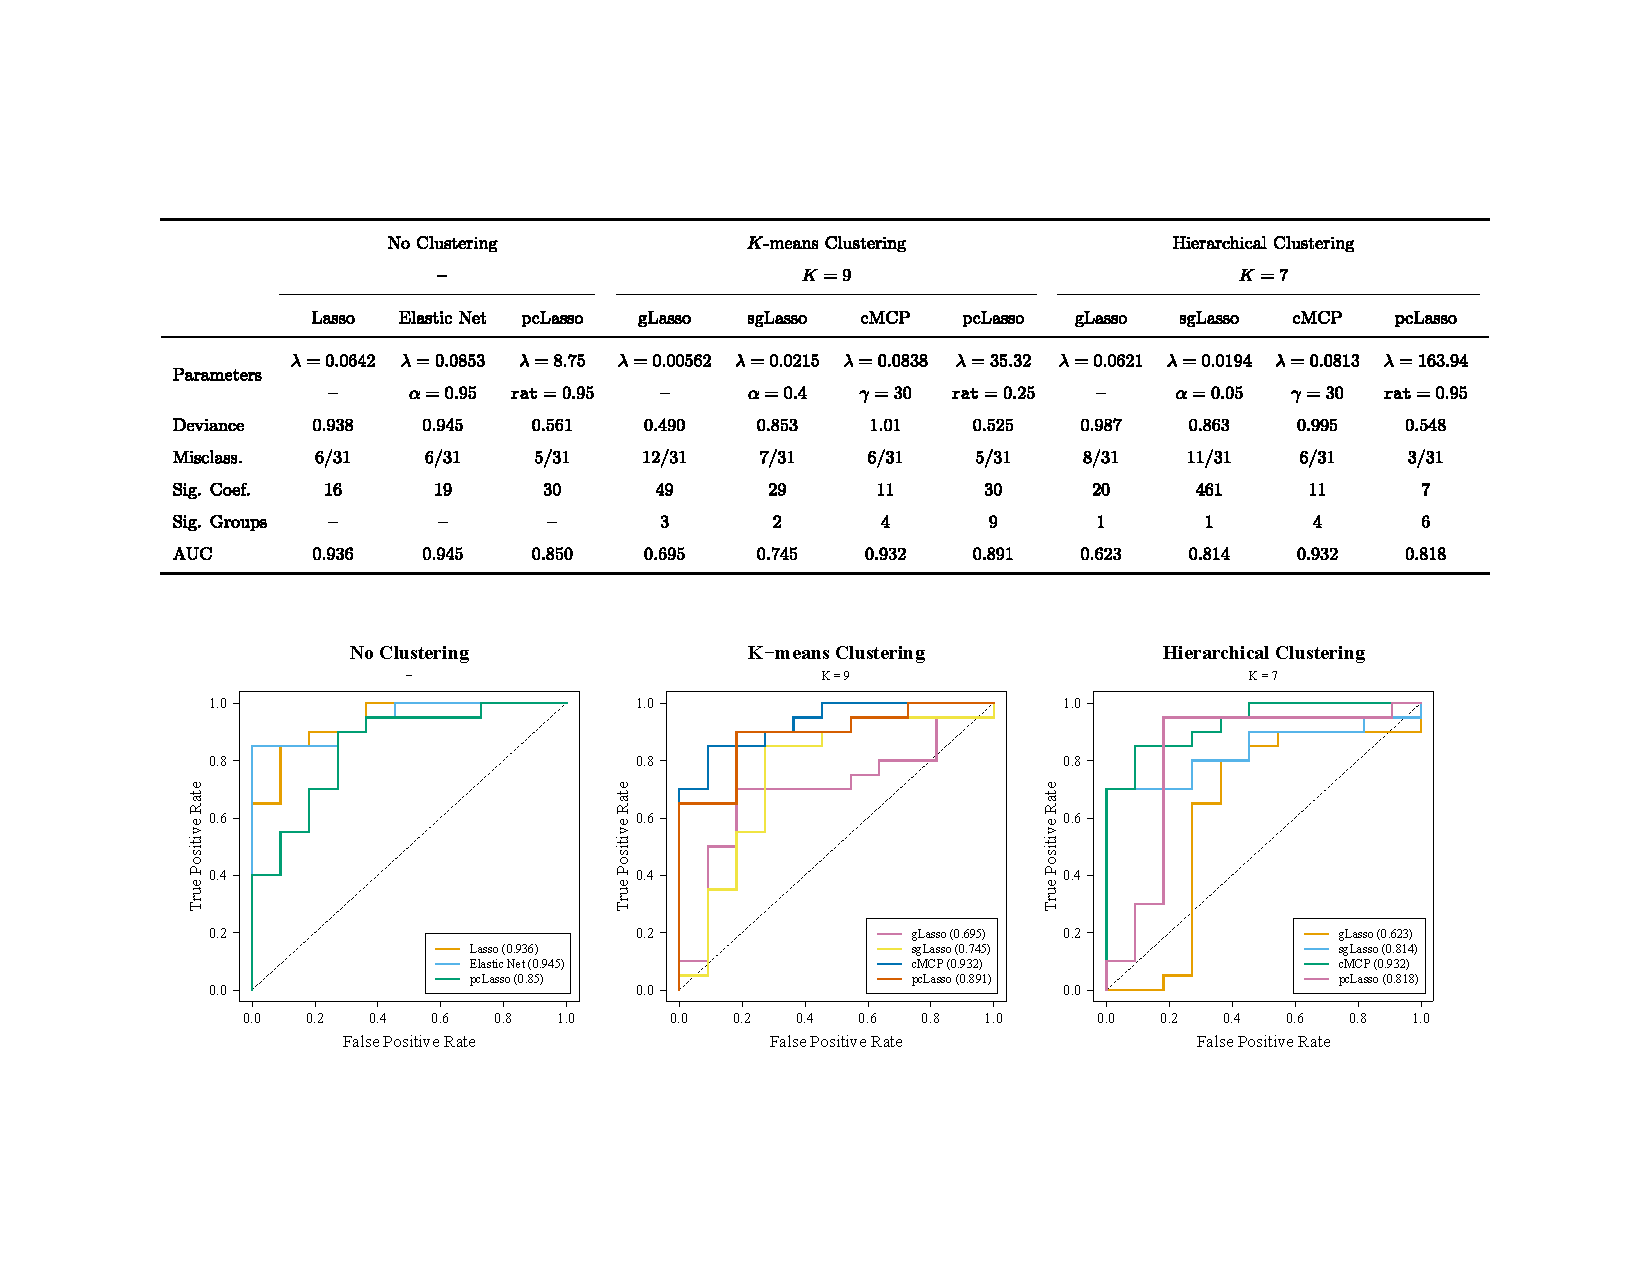
\includegraphics[trim = 75 100 75 100, clip, width = \textwidth]{colon_tab.pdf}
\end{center}
    
\end{frame}

\begin{frame}{$\ldots$}

\textbf{The winner}: pcLasso, both in terms of deviance and prediction accuracy.
\begin{itemize}
    \item The deviance for the non-group pcLasso is much lower than that of the lasso and the elastic net.
    \item The deviance for the group pcLasso is (generally) much lower than all of the other methods.
    \item Using hierarchical clustering, the pcLasso only misclassified 3 of the 31 test observations! %\Cooley[1.5][yellow]
\end{itemize} \mys

\textbf{Did clustering the predictors work?}: Not really!
\begin{itemize}
    \item The group lasso and sparse group lasso performed \textit{very poorly} for both clustering methods.
    \item \textit{This is an indication that the groups are not well-represented}.
    \item \textit{However}, pcLasso actually \textit{improves} when clustering is used!
\end{itemize}
    
\end{frame}

\begin{frame}{Future work}

We are currently working on a simulation study. We want to determine:
\begin{itemize}
    \item If pcLasso will always improve using clustered predictors.
    \item If $K$-means clustering with the GAP statistic is able to correctly identify the true underlying grouping structure in different situations.
    \item If very large $P$ will cause the GAP statistic to choose very large $K$.
\end{itemize} \mys

There are several avenues of research one could follow from our report:
\begin{itemize}
    \item pcLasso is a brand-new method (October 2018), and many of its theoretical properties have not been seen in practice.
    \item Use of different clustering methods to group the predictors, and attempt to find an ``optimal'' clustering method.
    \item Use of different regularization techniques.
    \item Allow for overlapping groups; all group regularization methods allow for this!
\end{itemize}
    
\end{frame}


%\begin{frame}[allowframebreaks]{References}

%\bibliographystyle{apacite}
%\bibliography{REU_bib}
    
%\end{frame}









\end{document}




